\documentclass[11pt]{article}
\usepackage[a4paper,vmargin=1in,hmargin=0.8in]{geometry}
\usepackage{amsmath,amssymb}
\usepackage{booktabs}
\usepackage{graphicx}
\usepackage{float}
\usepackage{longtable}
\usepackage[font=small,labelfont=bf,skip=5pt]{caption}
\usepackage{xcolor}
% placeholder for a citation still to be added from the literature-review notes
\newcommand{\refneeded}[1]{\textcolor{red}{[ref: #1]}}
% key phrase in observations: bold italic
\newcommand{\key}[1]{\textbf{\textit{#1}}}
\usepackage[colorlinks=true,linkcolor=blue,urlcolor=blue,citecolor=blue]{hyperref}
\graphicspath{{figs/}}
\renewcommand{\arraystretch}{1.1}
\setlength{\parindent}{0pt}
\setlength{\parskip}{4pt}

\title{\vspace{-15mm}\textbf{Calibrating the intelligent-agent model to lane-free mixed traffic}}
\author{Smitali Bhandari \qquad Bhargava Rama Chilukuri\\[3pt]
\small Department of Civil Engineering, Indian Institute of Technology Madras\\[6pt]
\normalsize UGRP Technical Report}
\date{\today}

\begin{document}
\maketitle

\begin{abstract}
\noindent
Mixed traffic in India moves without lane discipline: vehicles of very
different sizes and abilities share the road and take any lateral position.
This report calibrates the intelligent-agent model (IAM), a two-dimensional
social-force extension of the intelligent driver model, to 781\,s of trajectory
data of vehicles in seven classes on a 204\,m road section. All vehicles
are simulated together from their measured entry states, with one parameter
vector per class, searched with CMA-ES, and an exit stop line taken from the
measured signal-like stops. Vehicles are split into training and held-out sets
within the same simulation. One-at-a-time sensitivity
profiles show that the fit is governed by the car-following parameters of the
largest classes, while the road-edge and lateral anisotropy parameters are
hardly constrained. The calibrated traffic forms queues at the right times and
places, but its lateral motion is a slow drift rather than the deliberate
sideways moves of real vehicles, which points to the missing lateral target in
the model equations.
\end{abstract}

\begin{center}\small
All code: \url{https://github.com/ilatims-b/iam}
\end{center}

\tableofcontents

%======================================================================
\section{Introduction}
\label{sec:intro}

\subsection{Literature review}
\label{sec:lit}
Traffic-flow models are commonly grouped by the level at which they describe
traffic (Figure~\ref{fig:lit}).
\begin{itemize}\setlength{\itemsep}{1pt}
\item \emph{Macroscopic} models treat traffic as a continuum and describe the
evolution of density, flow and mean speed along the road \cite{lw55,richards56}.
\item \emph{Mesoscopic} models describe traffic through distributions of
vehicles, for example of desired and actual speeds, rather than through single
vehicles or a continuum \cite{ph71}.
\item \emph{Microscopic} models describe the motion of each vehicle and its
interaction with its neighbours, and are the natural level for heterogeneous
traffic, where vehicle classes differ in size and behaviour.
\end{itemize}

Approaches to lane-free microscopic traffic are either analytical or data-driven.
The analytical approaches are:
\begin{itemize}\setlength{\itemsep}{1pt}
\item \emph{Velocity obstacles}: the velocity obstacle (VO) of vehicle $A$
induced by $B$ is the set of velocities of $A$ that lead to a collision with
$B$ within a time horizon, assuming $B$ keeps its velocity, and $A$ chooses a
velocity outside it \cite{vo98}. Reciprocal velocity obstacles (RVO) let both
agents share the avoidance, which removes the oscillations of VO when both
avoid at once \cite{rvo08}. Optimal reciprocal collision avoidance (ORCA)
replaces each obstacle by a half-plane of permitted velocities, so the new
velocity follows from a linear program \cite{orca11}. ORCA assumes holonomic
agents. Variants for road vehicles, such as AutoRVO, restrict the search to
the velocities a vehicle can reach under its acceleration and turning limits
and represent agents of different shapes, for dense heterogeneous traffic
\cite{autorvo18}.
\item \emph{Strip-based} models divide the road width into narrow longitudinal
strips. A vehicle occupies several strips and may have more than one vehicle
ahead, so the leader is taken as the closest of the possible leaders.
Car-following uses a safe speed derived from the gap needed to stop behind the
leader, and a vehicle moves strip by strip according to a benefit, the
difference of safe speeds between strips, discounted with the number of strips
to cross. This handles the multiple-leader problem only in part. The SiMTraM
model, built on SUMO, reproduced one-minute mean speeds on an Indian highway
better than the default SUMO model \cite{simtram15}.
\item \emph{Social-force} models write each road user's acceleration as a sum
of a driving force towards its desired speed and direction and repulsive forces
from other users and boundaries \cite{hm95}. The intelligent-agent model (IAM) \cite{iam} builds on the intelligent driver
model (IDM) \cite{idm} in this way, as a fully two-dimensional model.
\item \emph{Cellular automata} discretise the road into cells and update
vehicle positions by local rules \cite{ns92}, and have been extended to
heterogeneous traffic with vehicles occupying several cells \cite{mallikarjuna09}.
\end{itemize}
The data-driven approaches are:
\begin{itemize}\setlength{\itemsep}{1pt}
\item \emph{Classical machine learning}: manoeuvres are recognised with hidden
Markov models or support vector machines from relative position, speed and
acceleration. These methods need a
grid structure and hand-made features, which makes them hard to apply to
heterogeneous traffic.
\item \emph{Deep learning}: RobustTP predicts the trajectories of road agents
in dense heterogeneous traffic over 3 to 5\,s, end to end from RGB video
\cite{robusttp19}. It builds on TraPHic, a combined LSTM and convolutional
network that weights the interactions between road agents in dense
heterogeneous traffic \cite{traphic19}. Transformers have since replaced
recurrent and convolutional networks in many of these models: a vision
transformer can encode a rasterised bird's-eye view of the scene for
multi-modal trajectory prediction \cite{postnikov21}, and spatio-temporal
transformers predict the trajectories of heterogeneous traffic agents from their
class, shape and heading \cite{s2tnet21}.
\item \emph{Reinforcement learning}: vehicle control in lane-free traffic is
learned from a reward \cite{karalakou23}.
\end{itemize}

\begin{figure}[H]\centering
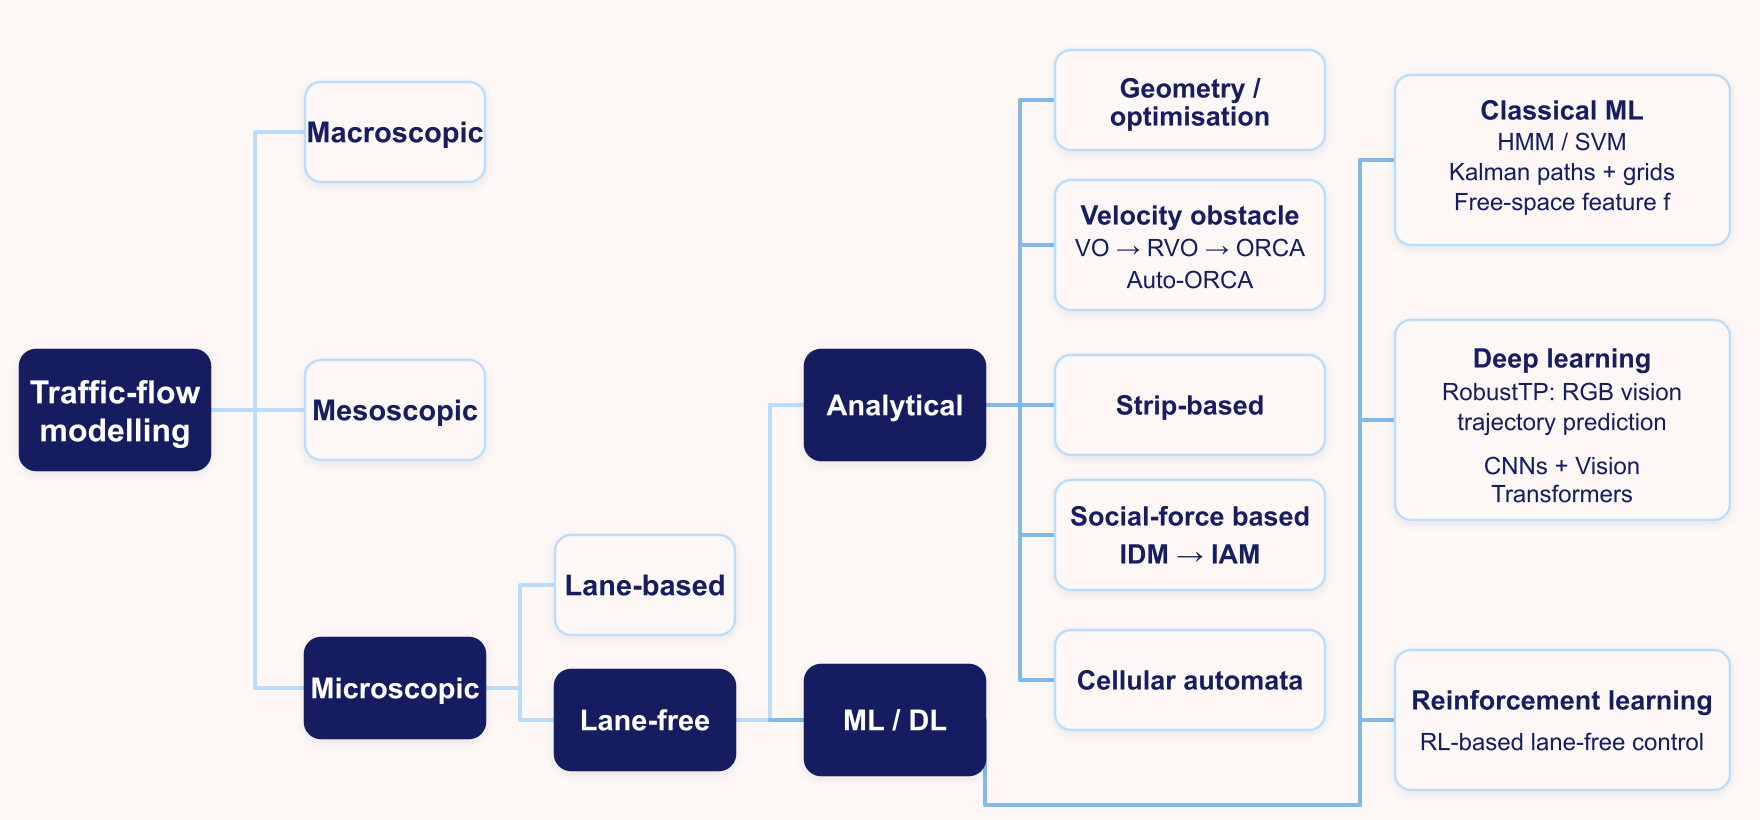
\includegraphics[width=\textwidth]{fig_litreview.png}
\caption{Approaches to traffic-flow modelling considered in this work. Dark
boxes: the path followed here, from microscopic and lane-free models to the
analytical, social-force based IAM.}
\label{fig:lit}
\end{figure}

\subsection{Choice of approach}
This work starts with an analytical approach, because an explicit model of
vehicle behaviour also builds a theoretical understanding of the problem. The
possible directions that follow from it are:
\begin{enumerate}\setlength{\itemsep}{1pt}
\item identifying the limitations of the chosen classical model;
\item a qualitative comparison of analytical approaches as a whole against
ML, DL and RL methods, for which
I have not found a benchmark or study in either Indian or Western settings;
\item extending the most physically grounded and adaptive approach.
\end{enumerate}
Among the analytical approaches, social-force models are the most intuitive,
and they had not yet been calibrated to lane-free traffic. We therefore work
with the IAM.

%======================================================================
\section{Our contribution}
\label{sec:contrib}
\begin{enumerate}\setlength{\itemsep}{2pt}
\item A calibration of the IAM to lane-free mixed traffic, with one parameter
vector for each of six vehicle classes (96 parameters), on trajectory data of
Indian mixed traffic, with quantitative errors on held-out vehicles. The IAM was
introduced with simulations of lane-based and lane-free traffic and a
comparison with naturalistic trajectories of one lane of an Athens arterial
from the pNEUMA drone data \cite{pneuma20}, which reproduces the observed
behaviour qualitatively and semi-quantitatively but reports no error measure;
validation on truly lane-free mixed traffic was left for future work
\cite{iam}. It had not been calibrated on Indian data.
\item A new simulation and train/test set-up for calibration. The whole record
is one simulation: every vehicle enters from its measured state and then runs on
its own simulated state, with simulated neighbours, for its whole time on the
section, and no trajectory is replayed. Vehicles are split into training and
held-out sets inside this one simulation, so held-out vehicles take part as
neighbours while their own errors are not used. Usual calibrations replay a
measured leader and split by leader-follower pair or platoon, and
multi-agent driving benchmarks split by whole scenario; we have not found a split
by vehicle within one simulation used for calibrating traffic models
(Section~\ref{sec:split}).

\item A comparison of the free calibration with runs in which the IDM
parameters are fixed at values calibrated elsewhere, as a single set and per
class, showing that such values do not transfer to this site
(Table~\ref{tab:runs}).
\item One-at-a-time sensitivity profiles of all 102 class parameters, showing
which parameters the data constrain and which they do not
(Figures~\ref{fig:key}--\ref{fig:Trmse} and Appendix~\ref{app:prof}).
\end{enumerate}

%======================================================================
\section{The intelligent-agent model}
\label{sec:model}

The intelligent-agent model (IAM) \cite{iam} is a two-dimensional microscopic
model: each vehicle has a longitudinal and a lateral equation of motion, and
there are no lanes. Each vehicle $i$ carries a longitudinal speed $v$ and a
lateral speed $w$. Its acceleration is the sum of a free term, interaction terms
from the neighbours ahead (leaders) and behind (followers), a road-edge term and,
laterally, a constant bias,
\begin{equation}
\begin{aligned}
\dot v_i&=g^{\mathrm{free}}+\min_{j\in\text{leaders}}f_{ij}
+\max_{k\in\text{followers}}p_{ik}+f^{B},\\
\dot w_i&=g^{\mathrm{self}}+\sum_{j\in\text{leaders}}g_{ij}
-\lambda_\perp\sum_{k\in\text{followers}}g_{ki}+g^{B}+\beta.
\end{aligned}
\label{eq:main}
\end{equation}
Neighbour $j$ is at $\Delta x=x_j-x_i$ and $\Delta y=y_j-y_i$, with
bumper-to-bumper gap $s=\max(\Delta x-L_j,0)$, mean width
$\overline W=\tfrac12(W_i+W_j)$ and side-to-side gap $s_y=|\Delta y|-\overline W$,
which is negative when the two bodies overlap laterally. All parameters are
listed in Table~\ref{tab:params}.

\subsection{Longitudinal dynamics}
Free acceleration follows the intelligent driver model (IDM) \cite{idm},
$g^{\mathrm{free}}=a\,[1-(v/v_0)^{\delta}]$, with $v_0$ the desired speed, $a$
the maximum acceleration and $\delta$ the acceleration exponent.

For the interaction we follow the authors' reference implementation, in which
the car-following term is the adaptive cruise control (ACC) model \cite{acc}.
ACC blends the IDM with a constant-acceleration heuristic (CAH) that uses the
leader's acceleration $a_l$. Writing $\Delta v=v-v_l$,
$\kappa=v_l\Delta v+2sa_l$ and $s^{*}=s_0+\max(0,\,vT+v\Delta v/2\sqrt{ab})$,
\begin{equation}
a_{\mathrm{IDM}}=a\Big[1-\big(\tfrac{v}{v_0}\big)^{\delta}-\big(\tfrac{s^{*}}{s}\big)^{2}\Big],
\label{eq:idm}
\end{equation}
\begin{equation}
\tilde a=\begin{cases}\dfrac{v^{2}a_l}{v_l^{2}-2sa_l}, & \kappa<0,\\[6pt]
a_l-\dfrac{\Delta v^{2}}{2\max(s,0.1)}\mathbb{1}_{\Delta v>0}, & \text{otherwise,}\end{cases}
\end{equation}
with $a_{\mathrm{CAH}}=\min(a,\tilde a)$ and
\begin{equation}
f^{\mathrm{CF}}=\max\!\big(-b_{\max},\;0.99\,a_{\mathrm{mix}}+0.01\,a_{\mathrm{IDM}}-g^{\mathrm{free}}\big),
\label{eq:acc}
\end{equation}
where $a_{\mathrm{mix}}=a_{\mathrm{IDM}}$ when $a_{\mathrm{IDM}}>a_{\mathrm{CAH}}$
and $a_{\mathrm{CAH}}+b\tanh[(a_{\mathrm{IDM}}-a_{\mathrm{CAH}})/b]$ otherwise.
The CAH handles cut-ins: when a vehicle moves into the gap ahead, the gap
collapses and the IDM alone would brake hard, although the new leader is not
braking and the gap will not shrink further. The retained one per cent of pure
IDM keeps its string stability.

The car-following force fades with the lateral offset of the leader and is
weaker when the two are side by side,
\begin{equation}
f_{ij}=\alpha_{\mathrm{long}}f^{\mathrm{CF}}_{ij},\qquad
\alpha_{\mathrm{long}}=\min\!\big(1,e^{-s_y/s_{0y}}\big)\times
\begin{cases}0.2, & \Delta x<L_j\text{ and }s_y>0,\\ 1, & \text{otherwise,}\end{cases}
\label{eq:flong}
\end{equation}
so $s_{0y}$ is the lateral width over which a leader stops mattering. Only the
strongest leader acts, through the $\min$ in~\eqref{eq:main}, so the
longitudinal force does not accumulate over neighbours. A follower $k$ close
behind the ego (gap below $0.5$\,m) that is braking because of it pushes it
forward by $p_{ik}=-\lambda_\parallel\,\alpha_{\mathrm{long}}f^{\mathrm{CF}}_{ki}\ge0$,
where $\lambda_\parallel$ is the longitudinal anisotropy.

\subsection{Lateral dynamics}
The lateral self term relaxes the lateral speed towards zero on a through
carriageway,
\begin{equation}
g^{\mathrm{self}}=-\frac{w}{\tau},
\label{eq:gself}
\end{equation}
with relaxation time $\tau$. \\
\textit{The model therefore has no notion of a vehicle
aiming for a lateral position: all lateral motion is a reaction to neighbours
and edges, followed by decay.}\\
 Each leader contributes a lateral desire
$\alpha_{ij}\in[-1,1]$ that points away from it,
\begin{equation}
\alpha_{ij}=-\mathrm{sgn}(\Delta y)\begin{cases}
|\Delta y|/\overline W, & |\Delta y|<\overline W,\\[3pt]
e^{-s_y/s_{0y,\mathrm{lat}}}, & \text{otherwise,}\end{cases}
\end{equation}
and a lateral acceleration
\begin{equation}
g_{ij}=-\frac{\sigma\,\alpha_{ij}\,f^{\mathrm{CF}}_{ij}}{\tau},\qquad |g_{ij}|\le4b.
\label{eq:gint}
\end{equation}
Since $f^{\mathrm{CF}}_{ij}<0$ for an interacting leader, $g_{ij}$ pushes the
ego away from $j$. The lateral sensitivity $\sigma$, in seconds, converts a
longitudinal force into a desired lateral speed, which the vehicle approaches
with time constant $\tau$; the lateral acceleration a neighbour causes is
therefore proportional to $\sigma/\tau$. Unlike the longitudinal case, every
interacting leader adds its own $g_{ij}$. A follower pushes the ego sideways in
the same way, scaled by the lateral anisotropy $\lambda_\perp$, except while the
lateral gap between the two is already opening. The constant $\beta$ is a
steady drift towards one side of the road.

\subsection{Road edges}
A vehicle near a road edge receives a restoring lateral acceleration that grows
linearly and without bound once the body is past the edge,
\begin{equation}
\alpha_{B,\mathrm{lat}}=\begin{cases}
e^{-s_y/s_{0y,\mathrm{lat}B}}, & s_y>0,\\[3pt]
1-s_y/s_{0y,\mathrm{lat}B}, & s_y\le0,\end{cases}
\qquad
g^{B}=g_B\,\big(\alpha_{B,\mathrm{lat}}^{\mathrm{right}}-\alpha_{B,\mathrm{lat}}^{\mathrm{left}}\big)\Big(0.2+0.8\,\frac{v}{v_{\mathrm{ref}}}\Big),
\label{eq:bnd}
\end{equation}
with $|g^{B}|\le20$\,m/s$^2$, where $s_y$ is the clear distance between the
vehicle's side and the nearer edge and $v_{\mathrm{ref}}=20$\,m/s is a fixed
reference speed from the reference code. The edge also slows the vehicle, by
$f^{B}=-f_B\,(\alpha^{\mathrm{left}}_{B}+\alpha^{\mathrm{right}}_{B})\,v/v_{\mathrm{ref}}$
with $\alpha_B=e^{-s_y/s_{0y,B}}$ (and $1$ past the edge). The edges are taken
from the data: the drivable span is $y\in[0,8.9]$\,m.

\subsection{Heading limit}
Lateral speed is limited through the heading angle $\theta=w/v$,
\begin{equation}
|\dot\theta|\le0.3\;\mathrm{s}^{-1},\qquad|\theta|\le0.3,\qquad|w|\le|\theta v|,
\label{eq:clamp}
\end{equation}
so the permitted lateral speed scales with the longitudinal speed and a
stopped vehicle cannot move sideways.

\subsection{Parameters}
Table~\ref{tab:params} lists the parameters. One vector of these parameters is
calibrated per vehicle class. 
% The IDM exponent $\delta$ is held at 4 in the
% free fit and set to the imported value in the fixed-IDM runs.

\begin{table}[H]\centering\footnotesize
\caption{Model parameters, calibrated per vehicle class.}
\label{tab:params}
\begin{tabular}{@{}llp{9.6cm}l@{}}
\toprule
& symbol & meaning & unit\\
\midrule
\multicolumn{4}{@{}l}{\emph{IDM}}\\
& $v_0$ & desired speed & m/s\\
& $T$ & desired time gap & s\\
& $s_0$ & minimum gap at standstill & m\\
& $a$ & maximum acceleration & m/s$^2$\\
& $b$ & comfortable deceleration & m/s$^2$\\
& $\delta$ & acceleration exponent & --\\
\midrule
\multicolumn{4}{@{}l}{\emph{IAM}}\\
& $s_{0y}$ & lateral width over which a leader's longitudinal force fades & m\\
& $s_{0y,\mathrm{lat}}$ & lateral width over which a leader's lateral push fades & m\\
& $\sigma$ & lateral sensitivity: longitudinal force to desired lateral speed & s\\
& $\tau$ & lateral relaxation time & s\\
& $\lambda_\parallel$ & longitudinal anisotropy: strength of a follower's forward push & --\\
& $\lambda_\perp$ & lateral anisotropy: strength of a follower's sideways push & --\\
& $\beta$ & constant lateral bias & m/s$^2$\\
& $f_B$ & longitudinal deceleration near a road edge & m/s$^2$\\
& $g_B$ & lateral acceleration away from a road edge & m/s$^2$\\
& $s_{0y,B}$ & width over which the edge's longitudinal effect fades & m\\
& $s_{0y,\mathrm{lat}B}$ & width over which the edge's lateral push fades & m\\
\bottomrule
\end{tabular}
\end{table}

\subsection{Vehicle dimensions}
Each class is a fixed rectangle (Table~\ref{tab:dims}); $L$ and $W$ are not
calibrated. The dimensions, like the trajectory data, were provided by Suhaib
Nazir, who is a Research Scholar in TR division (Acknowledgements). With these dimensions, the measured vehicle rectangles still
intersect on $3.0\,\%$ of vehicle-frames (against $4.3\,\%$ with the earlier
dimensions, Appendix~\ref{app:dims}), mostly between Bikes (Bike--Bike, Bike--Auto,
Bike--Truck) and between Trucks.

\begin{table}[H]\centering\footnotesize
\caption{Vehicle classes of the record (554 vehicles, 781\,s, 204\,m section)
and the dimensions used. Trailer has too few vehicles
for its own parameter vector and shares the MultiAxle vector.}
\label{tab:dims}
\begin{tabular}{@{}lrrrr@{}}
\toprule
class & vehicles & share & $L$ (m) & $W$ (m)\\
\midrule
Bike & 255 & 46.0\,\% & 1.8 & 0.65\\
Car & 125 & 22.6\,\% & 4.0 & 1.7\\
LCV & 66 & 11.9\,\% & 4.5 & 1.75\\
Truck & 51 & 9.2\,\% & 8.5 & 2.4\\
Auto & 33 & 6.0\,\% & 2.7 & 1.4\\
MultiAxle & 18 & 3.3\,\% & 12.0 & 2.5\\
Trailer & 6 & 1.1\,\% & 15.5 & 2.5\\
\bottomrule
\end{tabular}
\end{table}

%======================================================================
\section{Calibration}
\label{sec:calib}

\subsection{CMA-ES}
The parameters are searched with the covariance matrix adaptation evolution
strategy (CMA-ES) \cite{cma}, using the \texttt{pycma} implementation
\cite{pycma}. CMA-ES is derivative-free. CMA-ES suits this objective because it is not differentiable:
the $\min$ over leaders switches which neighbour acts, and the cap on $F$
creates flat regions.\\
It keeps a multivariate normal
distribution over the parameter vector, with mean $\mathbf m$, step size
$\sigma_{\mathrm{c}}$ and covariance $\mathbf C$, and each generation it
\begin{enumerate}\setlength{\itemsep}{1pt}
\item samples $\lambda$ candidates,
$\mathbf x_k=\mathbf m+\sigma_{\mathrm{c}}\,\mathbf y_k$, $\mathbf y_k\sim\mathcal N(\mathbf 0,\mathbf C)$,
$k=1,\dots,\lambda$;
\item evaluates the objective for each and ranks them, $\mathbf y_{1:\lambda}$
being the best;
\item moves the mean towards a weighted average of the best $\mu=\lfloor\lambda/2\rfloor$,
\begin{equation}
\mathbf m\leftarrow\mathbf m+\sigma_{\mathrm{c}}\,\langle\mathbf y\rangle_w,\qquad
\langle\mathbf y\rangle_w=\sum_{i=1}^{\mu}w_i\,\mathbf y_{i:\lambda},\quad
w_1\ge\dots\ge w_\mu>0,\ \textstyle\sum w_i=1;
\end{equation}
\item adapts the step size from the length of an evolution path
$\mathbf p_\sigma$, which accumulates successive steps,
\begin{equation}
\mathbf p_\sigma\leftarrow(1-c_\sigma)\mathbf p_\sigma
+\sqrt{c_\sigma(2-c_\sigma)\mu_{\mathrm{eff}}}\;\mathbf C^{-1/2}\langle\mathbf y\rangle_w,\qquad
\sigma_{\mathrm{c}}\leftarrow\sigma_{\mathrm{c}}\exp\!\Big(\frac{c_\sigma}{d_\sigma}\Big(\frac{\|\mathbf p_\sigma\|}{\mathrm E\|\mathcal N(\mathbf 0,\mathbf I)\|}-1\Big)\Big),
\end{equation}
so the step grows when successive steps point the same way and shrinks when
they cancel;
\item adapts the covariance from a second path $\mathbf p_c$ (rank-one update)
and from the selected steps themselves (rank-$\mu$ update),
\begin{equation}
\mathbf C\leftarrow(1-c_1-c_\mu)\,\mathbf C+c_1\,\mathbf p_c\mathbf p_c^{\top}
+c_\mu\sum_{i=1}^{\mu}w_i\,\mathbf y_{i:\lambda}\mathbf y_{i:\lambda}^{\top},
\end{equation}
so that the distribution stretches along directions in which the objective
keeps improving.
\end{enumerate}
Here $\mu_{\mathrm{eff}}=1/\sum w_i^2$, and the learning rates $c_\sigma$,
$d_\sigma$, $c_1$, $c_\mu$, $c_c$ take their default values, which depend only
on the dimension $n$ and on $\mu_{\mathrm{eff}}$ \cite{cma}:
\begin{equation}
\begin{gathered}
c_\sigma=\frac{\mu_{\mathrm{eff}}+2}{n+\mu_{\mathrm{eff}}+5},\qquad
c_c=\frac{4+\mu_{\mathrm{eff}}/n}{n+4+2\mu_{\mathrm{eff}}/n},\\
c_1=\frac{2}{(n+1.3)^2+\mu_{\mathrm{eff}}},\qquad
c_\mu=\min\!\Big(1-c_1,\ \frac{2(\mu_{\mathrm{eff}}-2+1/\mu_{\mathrm{eff}})}{(n+2)^2+\mu_{\mathrm{eff}}}\Big),
\end{gathered}
\end{equation}
and $d_\sigma=1+2\max\big(0,\sqrt{(\mu_{\mathrm{eff}}-1)/(n+1)}-1\big)+c_\sigma$.
The step-size and path rates thus scale as $c_\sigma,c_c=O(1/n)$ and the
covariance rates as $c_1=O(1/n^2)$ and $c_\mu=O(\mu_{\mathrm{eff}}/n^2)$, so the
covariance matrix needs of the order of $n^2/\mu_{\mathrm{eff}}$ generations to
adapt. The population is $\lambda=4+\lfloor3\ln n\rfloor$ and $\mu=\lfloor\lambda/2\rfloor$:
for the 96 parameters of the free fit $\lambda=17$, $\mu=8$, $\mu_{\mathrm{eff}}=5.1$,
$c_\sigma=0.067$, $c_c=0.041$, $c_1=2.1\times10^{-4}$ and $c_\mu=6.9\times10^{-4}$;
for the 66 parameters of the fixed-IDM fits $\lambda=16$, $c_1=4.4\times10^{-4}$
and $c_\mu=1.3\times10^{-3}$. With about 1\,300 generations in two hours, the
free fit is of the same order as $n^2/\mu_{\mathrm{eff}}\approx1\,800$, so the
covariance has only partly adapted by the time the run stops.

\subsection{Objective and search space}
For one vehicle trace, with $\hat\cdot$ denoting simulated quantities,
\begin{equation}
F=\frac{\mathrm{RMSE}(x)}{x_{\mathrm{sc}}}
+\frac{\mathrm{RMSE}(y)}{y_{\mathrm{sc}}}
+\frac{\mathrm{RMSE}(v)}{\max(\mathrm{RMS}(v_{\mathrm{obs}}),0.5)},
\qquad x_{\mathrm{sc}}=2.0\ \mathrm m,\ y_{\mathrm{sc}}=0.5\ \mathrm m.
\label{eq:F}
\end{equation}
The two position terms use fixed scales, so that a metre of error counts the
same for every vehicle; the speed term is relative to the vehicle's own speed.
The objective minimised is the mean of $F$ over the training vehicles, each
capped at $F=60$ so that a few diverging vehicles cannot dominate. Traces
shorter than 50 frames (2\,s) are not scored.

\begin{itemize}
    \item The search runs in a normalised box $z\in[0,10]^n$, each coordinate mapped
linearly or logarithmically onto the parameter's search box
(Table~\ref{tab:bounds}).
\item 
 Bounds are enforced by the \texttt{pycma}
\texttt{BoundTransform}. The boxes were chosen from what drivers can do and
from the measured traffic, by class:
\begin{itemize}
    \item  positive acceleration 99th percentile
0.7--1.3\,m/s$^2$, braking 99th percentile 1.4--2.0\,m/s$^2$,
    \item  median standstill
gap 1.0--2.3\,m,
\item 5th percentile of the moving time headway 0.33--1.6\,s,
\item lateral speed 99th percentile 0.1--1.0\,m/s, free-flow 85th percentile speed
8--13\,m/s.
\item  Widths stop at the precision of smoothed video tracks rather than at
a few centimetres.
\end{itemize} 
\item The search is continuous: CMA-ES draws real-valued candidates from its
normal distribution, so any value inside the box can be tried, and nothing is
rounded. Rounding would make the objective constant between grid points, and
CMA-ES, which adapts its step size and covariance from small differences in
$F$, would stall.
\item The \emph{granularity} of a parameter (Table~\ref{tab:bounds}) is the
smallest change in it that we treat as meaningful, either for a driver (for
example $0.1$\,s of time gap or $0.5$\,m/s of desired speed) or given the
precision of the smoothed trajectories (for widths, $0.05$\,m). It is not used
by the search; it sets the step of the sensitivity profiles and the precision
with which fitted values are reported. Every run starts from the values in the ``start''
column, with $v_0$ seeded per class from the free-flow speed (85th percentile of
speed in the least dense tenth of frames.)
\end{itemize}

\begin{table}[H]\centering\footnotesize
\caption{Search box, scale, starting value and granularity of every
parameter. $^{a}$\,Free-flow speed of the class.}
\label{tab:bounds}
\begin{tabular}{@{}llllll@{}}\toprule
parameter & unit & search box & scale & start & granularity\\\midrule
\multicolumn{6}{@{}l}{\emph{IDM (car-following core)}}\\
$v_0$ & m/s & [5, 25] & linear & per class$^{a}$ & 0.5 m/s\\
$T$ & s & [0.2, 3] & linear & 1.2 & 0.1 s\\
$s_0$ & m & [0.2, 4] & linear & 1.5 & 0.1 m\\
$a$ & m/s$^2$ & [0.3, 3] & linear & 1 & 0.1 m/s$^2$\\
$b$ & m/s$^2$ & [0.5, 3] & linear & 1.5 & 0.1 m/s$^2$\\
$\delta$ & -- & [3, 6] & linear & 4 & 0.1 \\
\multicolumn{6}{@{}l}{\emph{IAM (lateral, anisotropy, bias, road edge)}}\\
$s_{0y}$ & m & [0.1, 2] & log & 0.1 & 0.05 m\\
$s_{0y,\mathrm{lat}}$ & m & [0.1, 2] & log & 0.15 & 0.05 m\\
$\sigma$ & s & [0.01, 2] & log & 1 & 10\,\%\\
$\tau$ & s & [0.2, 5] & log & 1 & 0.1 s\\
$\lambda_\parallel$ & -- & [0, 0.6] & linear & 0.1 & 0.05 \\
$\lambda_\perp$ & -- & [0, 0.6] & linear & 0.1 & 0.05 \\
$\beta$ & m/s$^2$ & [-0.2, 0.2] & linear & 0 & 0.01 m/s$^2$\\
$f_B$ & m/s$^2$ & [0, 1] & linear & 0.2 & 0.05 m/s$^2$\\
$g_B$ & m/s$^2$ & [0.1, 2] & linear & 2 & 0.1 m/s$^2$\\
$s_{0y,B}$ & m & [0.05, 1] & log & 0.1 & 0.05 m\\
$s_{0y,\mathrm{lat}B}$ & m & [0.05, 1] & log & 0.1 & 0.05 m\\
\bottomrule\end{tabular}

\end{table}
\subsection{Dataset}
The trajectory data and the vehicle dimensions were provided by Suhaib Nazir
(Acknowledgements). The record covers 781\,s of traffic on a 204\,m section of
an 8.7\,m carriageway without lane discipline, with 554 vehicles in seven
classes (Table~\ref{tab:dims}) and one row per vehicle per 0.04\,s frame,
830\,240 vehicle-frames in all. Table~\ref{tab:cols} lists the columns and how
each is used, and Table~\ref{tab:stats} summarises the traffic. The traffic is
mostly congested: the median longitudinal speed is 2.1\,m/s against a maximum of
21.8\,m/s, and on $36\,\%$ of vehicle-frames vehicles move slower than 0.5\,m/s.

\begin{table}[H]\centering\footnotesize
\caption{Columns of the dataset and how each is used. ``Entry state'': read
once, at the frame the vehicle first appears; ``scoring'': compared with the
simulation afterwards.}
\label{tab:cols}
\begin{tabular}{@{}lll@{}}
\toprule
column & content & use\\
\midrule
\texttt{VehicleID}, \texttt{Class} & identifier, vehicle class & grouping, class parameters\\
\texttt{Time} & time since the vehicle's first frame (s) & not used\\
\texttt{GTime\_sec} & global time stamp (s) & common frame index\\
\texttt{X}, \texttt{Y} & raw position (m) & not used\\
\texttt{X\_Smt}, \texttt{Y\_Smt} & smoothed centroid position (m) & entry state, scoring\\
\texttt{Long\_Speed}, \texttt{Lat\_Speed} & speed along and across the road (m/s) & entry state, scoring\\
\texttt{Speed} & total speed (m/s) & not used\\
\texttt{Long\_Acc} & longitudinal acceleration (m/s$^2$) & entry state\\
\texttt{Lat\_Acc} & lateral acceleration (m/s$^2$) & summary statistics only\\
\texttt{Acceleration} & total acceleration (m/s$^2$) & not used\\
\bottomrule
\end{tabular}
\end{table}

\begin{table}[H]\centering\footnotesize
\caption{Summary of the measured traffic over all vehicle-frames. Occupancy:
number of vehicles on the section at one frame.}
\label{tab:stats}
\begin{tabular}{@{}lr@{}}
\toprule
quantity & value\\
\midrule
vehicle-frames & 830\,240\\
median / mean longitudinal speed & 2.11 / 3.03\,m/s\\
maximum longitudinal speed & 21.8\,m/s\\
free-flow speed (85th percentile, least dense tenth of frames) & 8.0--13.2\,m/s by class\\
mean occupancy & 42.5 vehicles (0.21 per m)\\
share of vehicle-frames below 0.5\,m/s & $36\,\%$\\
standard deviation of longitudinal / lateral acceleration & 0.490 / 0.080\,m/s$^2$\\
\bottomrule
\end{tabular}
\end{table}

\subsection{Simultaneous simulation}
The whole 781\,s record is simulated. All 554
vehicles are integrated forward together at $\mathrm{d}t=0.04$\,s, the
sampling interval. A vehicle enters at the first frame on which it appears in
the record, with its measured position, speed and acceleration, and from then
on it runs on its own simulated state until it leaves the section. Its
neighbours are the other simulated vehicles, at their simulated positions.
Three things come from the record: each vehicle's state at entry, its class and
dimensions, and its measured trajectory, used to score the result. Each vehicle
is predicted over its whole time on the section [a median of 52\,s and up to
171\,s.]

The downstream end of the section is held by a virtual stop line during the
six periods in which the measured traffic at the exit is stopped (71--114,
216--274, 356--416, 503--521, 530--563 and 660--698\,s). It is a stopped
obstacle across the road at 202.1\,m, holds every class except Bike, and acts
only longitudinally. The evidence that the queues are caused by a signal beyond/at
the exit is summarised in Appendix~\ref{app:signal}.

\subsection{Train/test split by vehicle}
\label{sec:split}
Vehicles are split into training and held-out sets within the same simulation.
Within each class, vehicles are ordered by entry time and cut into groups of
ten, and three of each group are held out at random: 387 training and 167
held-out vehicles. Held-out vehicles are simulated like every other vehicle and
act as neighbours of training vehicles, but their errors never enter the
objective. The split therefore tests transfer to other vehicles in the same
traffic, not to another period.

The usual practice in car-following calibration is different. In local
(leader-follower) calibration the leader's measured trajectory is replayed and
only the follower is simulated, and validation uses other pairs \cite{kt08};
platoon calibration simulates a few followers behind a replayed leader and
validates on other platoons \cite{kurtc16}. In both, train and test are
separate sets of trajectories, and the test vehicles never interact with the
training vehicles. Closed-loop simulation of all agents of a scene is used for
autonomous-driving benchmarks such as the Waymo Open Sim Agents Challenge, but
there the split is by whole scenario \cite{wosac23}. Here nothing is replayed:
every vehicle is simulated, and the split is by vehicle inside one simulation,
so held-out vehicles take part as neighbours while their own errors are not
used. We have not found this split used for calibrating traffic models. The
closest analogue is the transductive node split of semi-supervised learning on
graphs \cite{kipf17}, in which all nodes are present during training but only
the labels of the training nodes enter the loss. The same caveat applies: the
held-out score measures transfer to other vehicles in the same traffic, and is
likely optimistic for other periods or sites.

\subsection{Reported errors}
Errors are reported as pooled RMSE over all data points of a set of vehicles, a
data point being one vehicle at one frame,
\begin{equation}
\mathrm{RMSE}_{\mathrm{pooled}}(x)=\sqrt{\frac{\sum_{i}\sum_{t\in\mathcal T_i}\big(\hat x_{i,t}-x_{i,t}\big)^{2}}{\sum_{i}|\mathcal T_i|}}
=\sqrt{\frac{\sum_i n_i\,\mathrm{RMSE}_i(x)^{2}}{\sum_i n_i}},
\label{eq:pooled}
\end{equation}
where $i$ runs over the vehicles of the set, $\mathcal T_i$ is the set of
frames on which vehicle $i$ is scored and $n_i=|\mathcal T_i|$. The same
formula gives the lateral ($y$) and speed ($v$) errors. The objective $F$ is
reported as its mean over the vehicles of the set. 386 training and 165
held-out vehicles have at least 50 frames and are scored.

\subsection{Runs}
Three runs are compared. All use the stop line, the search boxes of
Table~\ref{tab:bounds}, the dimensions of Table~\ref{tab:dims} and the same
split.
\begin{enumerate}\setlength{\itemsep}{1pt}
\item \emph{Fixed IDM, single set.} One IDM parameter set for every class
\cite{chandra} ($v_0=18.76$\,m/s, $T=0.89$\,s, $s_0=1.05$\,m, $a=2.0$\,m/s$^2$,
$b=2.63$\,m/s$^2$, $\delta=4.42$); the 11 IAM parameters per class are
calibrated (66 values).
\item \emph{Fixed IDM, per class.} IDM parameters per class from the pairwise
calibration of \cite[slide~10]{duggal} for Auto, Bike and Car, extrapolated for LCV,
Truck and MultiAxle (Appendix~\ref{app:idm}); the IAM parameters are calibrated
(66 values).
\item \emph{All parameters free.} The five IDM parameters $v_0,T,s_0,a,b$ and
the 11 IAM parameters are calibrated per class (96 values); $\delta=4$.
\end{enumerate}

\begin{table}[H]\centering\footnotesize
\caption{Mean $F$ and pooled RMSE~\eqref{eq:pooled} of position along the
road (long.), position across it (lat.) and speed, for the three runs and for
a constant-velocity baseline, in which each vehicle keeps its measured entry
speed, along and across the road, for its whole time on the section; the
baseline is scored on the same vehicles and frames. Per-class values are in
Appendix~\ref{app:cls}.}
\label{tab:runs}
\begin{tabular}{@{}l rrrr rrrr@{}}\toprule
 & \multicolumn{4}{c}{training vehicles (386)} & \multicolumn{4}{c}{held-out vehicles (165)}\\
\cmidrule(lr){2-5}\cmidrule(l){6-9}
run & $F$ & long.\ (m) & lat.\ (m) & speed (m/s) & $F$ & long.\ (m) & lat.\ (m) & speed (m/s)\\\midrule
Fixed IDM, single set \cite{chandra} & 20.06 & 35.1 & 1.89 & 6.97 & 20.20 & 35.5 & 1.73 & 6.35\\
Fixed IDM, per class \cite{duggal} & 26.03 & 47.5 & 1.76 & 11.35 & 27.35 & 49.3 & 1.65 & 10.87\\
All parameters free & 12.52 & 22.3 & 1.47 & 2.86 & 12.19 & 22.4 & 1.51 & 2.60\\
\midrule
Constant velocity & 48.27 & 294.8 & 6.77 & 7.25 & 47.21 & 326.8 & 6.11 & 7.70\\
\bottomrule\end{tabular}

\end{table}

\paragraph{Observations.}
\begin{itemize}\setlength{\itemsep}{1pt}
\item The \key{free fit has the lowest errors on every measure}: held-out pooled
RMSE of 22.4\,m along the road, 1.51\,m across it and 2.60\,m/s in speed,
against 326.8\,m, 6.11\,m and 7.70\,m/s for constant velocity. Even the worst
run reduces the baseline's longitudinal error by a factor of about seven.
\item \key{Fixing the IDM at imported values raises the errors}: with the single
set the held-out longitudinal error is 35.5\,m and the speed error 6.35\,m/s;
with the per-class values 49.3\,m and 10.87\,m/s.
\item The cause is the \key{imported desired speeds} ($v_0=16$--21\,m/s), which
lie far above the speeds of this record (free-flow 85th percentile
8--13\,m/s); no setting of the IAM parameters compensates.
\item In every run the training and held-out errors are close, so the fits
do not over-fit the training vehicles.
\end{itemize}

\begin{table}[H]\centering\footnotesize
\caption{Class parameters of the run with IDM fixed at a single set \cite{chandra}.
Italic: fixed, not calibrated. Trailer uses the MultiAxle column.}
\label{tab:parchandra}
\begin{tabular}{@{}lrrrrrr@{}}\toprule
parameter & Auto & Bike & Car & LCV & Truck & MultiAxle\\\midrule
\multicolumn{7}{@{}l}{\emph{IDM}}\\
$v_0$ & \textit{18.76} & \textit{18.76} & \textit{18.76} & \textit{18.76} & \textit{18.76} & \textit{18.76}\\
$T$ & \textit{0.89} & \textit{0.89} & \textit{0.89} & \textit{0.89} & \textit{0.89} & \textit{0.89}\\
$s_0$ & \textit{1.05} & \textit{1.05} & \textit{1.05} & \textit{1.05} & \textit{1.05} & \textit{1.05}\\
$a$ & \textit{2.00} & \textit{2.00} & \textit{2.00} & \textit{2.00} & \textit{2.00} & \textit{2.00}\\
$b$ & \textit{2.63} & \textit{2.63} & \textit{2.63} & \textit{2.63} & \textit{2.63} & \textit{2.63}\\
$\delta$ & \textit{4.42} & \textit{4.42} & \textit{4.42} & \textit{4.42} & \textit{4.42} & \textit{4.42}\\
\multicolumn{7}{@{}l}{\emph{IAM}}\\
$s_{0y}$ & 1.74 & 2.00 & 1.28 & 0.89 & 1.42 & 0.72\\
$s_{0y,\mathrm{lat}}$ & 0.72 & 0.18 & 0.23 & 0.53 & 1.98 & 0.21\\
$\sigma$ & 0.053 & 0.034 & 0.013 & 0.015 & 0.028 & 0.011\\
$\tau$ & 1.58 & 0.53 & 0.41 & 0.33 & 0.94 & 1.09\\
$\lambda_\parallel$ & 0.59 & 0.59 & 0.21 & 0.49 & 0.11 & 0.31\\
$\lambda_\perp$ & 0.23 & 0.36 & 0.51 & 0.38 & 0.19 & 0.60\\
$\beta$ & 0.004 & -0.18 & -0.19 & 0.070 & -0.11 & -0.037\\
$f_B$ & 0.30 & 0.95 & 0.99 & 0.15 & 0.39 & 0.24\\
$g_B$ & 1.35 & 1.93 & 1.43 & 0.55 & 1.51 & 0.70\\
$s_{0y,B}$ & 1.00 & 0.98 & 1.00 & 0.72 & 0.054 & 0.91\\
$s_{0y,\mathrm{lat}B}$ & 0.44 & 0.63 & 0.77 & 0.35 & 0.30 & 0.38\\
\bottomrule\end{tabular}

\end{table}
\begin{table}[H]\centering\footnotesize
\caption{Class parameters of the run with IDM fixed per class at the values
of \cite{duggal} (Auto, Bike, Car) and extrapolated values (LCV, Truck, MultiAxle).
Italic: fixed, not calibrated.}
\label{tab:parduggal}
\begin{tabular}{@{}lrrrrrr@{}}\toprule
parameter & Auto & Bike & Car & LCV & Truck & MultiAxle\\\midrule
\multicolumn{7}{@{}l}{\emph{IDM}}\\
$v_0$ & \textit{20.27} & \textit{21.28} & \textit{21.43} & \textit{20.00} & \textit{18.00} & \textit{16.00}\\
$T$ & \textit{0.31} & \textit{0.25} & \textit{0.29} & \textit{0.31} & \textit{0.36} & \textit{0.42}\\
$s_0$ & \textit{0.64} & \textit{1.04} & \textit{1.00} & \textit{1.10} & \textit{1.30} & \textit{1.50}\\
$a$ & \textit{2.57} & \textit{1.86} & \textit{2.09} & \textit{1.90} & \textit{1.84} & \textit{1.46}\\
$b$ & \textit{0.93} & \textit{1.28} & \textit{1.35} & \textit{1.12} & \textit{1.15} & \textit{1.05}\\
$\delta$ & \textit{4.50} & \textit{4.43} & \textit{4.33} & \textit{4.33} & \textit{4.33} & \textit{4.33}\\
\multicolumn{7}{@{}l}{\emph{IAM}}\\
$s_{0y}$ & 0.57 & 1.98 & 1.98 & 1.98 & 0.96 & 1.68\\
$s_{0y,\mathrm{lat}}$ & 0.10 & 0.15 & 0.31 & 0.21 & 0.17 & 0.30\\
$\sigma$ & 0.35 & 0.020 & 0.016 & 0.013 & 0.017 & 0.015\\
$\tau$ & 2.21 & 4.43 & 0.28 & 0.41 & 1.56 & 0.78\\
$\lambda_\parallel$ & 0.24 & 0.000 & 0.003 & 0.14 & 0.008 & 0.076\\
$\lambda_\perp$ & 0.17 & 0.19 & 0.26 & 0.007 & 0.60 & 0.31\\
$\beta$ & -0.032 & -0.019 & 0.11 & 0.083 & 0.062 & -0.17\\
$f_B$ & 0.26 & 0.14 & 0.21 & 0.66 & 0.017 & 1.00\\
$g_B$ & 1.15 & 1.96 & 1.78 & 1.25 & 1.84 & 1.56\\
$s_{0y,B}$ & 0.13 & 0.17 & 0.24 & 0.14 & 0.94 & 0.81\\
$s_{0y,\mathrm{lat}B}$ & 0.24 & 1.00 & 0.059 & 0.19 & 0.97 & 0.088\\
\bottomrule\end{tabular}

\end{table}

\begin{table}[H]\centering\footnotesize
\caption{Class parameters of the run with all parameters free. Italic: fixed
($\delta$).}
\label{tab:parfree}
\begin{tabular}{@{}lrrrrrr@{}}\toprule
parameter & Auto & Bike & Car & LCV & Truck & MultiAxle\\\midrule
\multicolumn{7}{@{}l}{\emph{IDM}}\\
$v_0$ & 11.95 & 5.00 & 5.65 & 7.57 & 11.34 & 14.38\\
$T$ & 0.25 & 0.26 & 0.82 & 2.06 & 0.60 & 2.02\\
$s_0$ & 1.45 & 0.65 & 0.30 & 0.62 & 1.13 & 0.34\\
$a$ & 1.37 & 0.30 & 1.56 & 1.35 & 0.81 & 2.35\\
$b$ & 2.39 & 1.66 & 0.50 & 0.53 & 2.99 & 0.90\\
$\delta$ & \textit{4.00} & \textit{4.00} & \textit{4.00} & \textit{4.00} & \textit{4.00} & \textit{4.00}\\
\multicolumn{7}{@{}l}{\emph{IAM}}\\
$s_{0y}$ & 0.14 & 0.10 & 1.99 & 1.69 & 1.11 & 0.50\\
$s_{0y,\mathrm{lat}}$ & 0.49 & 0.22 & 0.44 & 0.22 & 0.40 & 0.40\\
$\sigma$ & 0.11 & 0.71 & 0.010 & 0.011 & 0.89 & 0.042\\
$\tau$ & 3.23 & 0.95 & 0.25 & 0.23 & 2.82 & 0.85\\
$\lambda_\parallel$ & 0.20 & 0.13 & 0.18 & 0.27 & 0.13 & 0.30\\
$\lambda_\perp$ & 0.11 & 0.28 & 0.60 & 0.046 & 0.55 & 0.57\\
$\beta$ & 0.025 & 0.18 & 0.046 & 0.055 & -0.14 & -0.13\\
$f_B$ & 0.26 & 0.96 & 0.086 & 0.79 & 0.97 & 0.36\\
$g_B$ & 1.22 & 0.66 & 0.44 & 1.53 & 0.32 & 0.87\\
$s_{0y,B}$ & 0.39 & 0.076 & 0.16 & 0.057 & 0.44 & 0.053\\
$s_{0y,\mathrm{lat}B}$ & 0.77 & 0.47 & 0.42 & 0.12 & 0.85 & 0.73\\
\bottomrule\end{tabular}

\end{table}

\paragraph{Observations.}
\begin{itemize}\setlength{\itemsep}{1pt}
\item The fitted desired speed is low, 5.0--14.4\,m/s, in line with the
congested record.
\item Several values sit \key{at a bound}: Bike's $v_0$ (5\,m/s) and maximum
acceleration ($a=0.30$\,m/s$^2$), and Car's comfortable deceleration
($b=0.50$\,m/s$^2$).
\item For Car and LCV, $\sigma$ is at its lower bound and $\tau$ close to it, so
their \key{lateral push from leaders is almost switched off}; Bike and Truck keep
a clearly non-zero $\sigma$.
\item The \key{time gap differs strongly between classes}, from 0.25--0.26\,s
for Auto and Bike to about 2\,s for LCV and MultiAxle.
\end{itemize}

\subsection{Sensitivity analysis}
The sensitivity of the free fit is examined with one-at-a-time profiles; variance-based methods \cite{punzo} would also capture interactions between parameters, at a much higher cost. For
each class vector and each parameter, the parameter is moved across its search
box in steps of its granularity (Table~\ref{tab:bounds}, at most 60 points),
with every other parameter held at the fitted value, and the whole record is
simulated again. The curve of $F$ against the value of one parameter of one
class obtained this way is called a \emph{profile}; there are 102 profiles
(17 parameters for 6 class vectors) and 3\,151 simulations in all.
Figure~\ref{fig:key} shows the profiles of the six parameters with the largest
effect on $F$, Figure~\ref{fig:weak} six that the data hardly constrain, and
Figure~\ref{fig:Trmse} how the three pooled RMSEs respond to the time gap. All
102 profiles, for $F$ and for each pooled RMSE, and a summary of each profile as
the distribution of $F$ over all values tried, are in Appendix~\ref{app:prof}.

The simulation is deterministic, so the same parameters always give the same
$F$. Even so, $F$ is not smooth along a profile. A small change in one
parameter can decide, for example, whether a vehicle enters a gap before a
queue closes; the change then passes to its neighbours and on through the
traffic over 781\,s, so $F$ moves in small jumps rather than smoothly. We
measure this roughness as the median absolute difference of $F$ between
neighbouring points of a profile: 0.24, or $1.9\,\%$ of the fitted $F$. A
parameter whose profile varies by no more than a few such jumps over its whole
box (a range below about 1.5) cannot be told apart from this roughness.
\begin{figure}[H]\centering
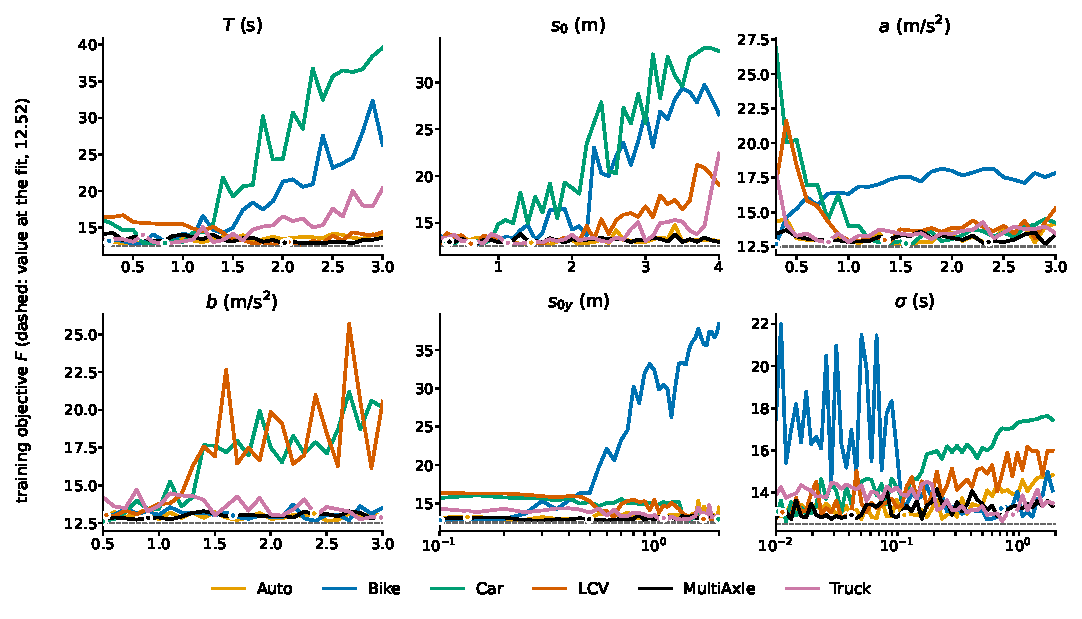
\includegraphics[width=\textwidth]{fig_oat_key.pdf}
\caption{Profiles of the six parameters with the largest effect on the fit:
training objective $F$ against the value of one parameter, one line per class,
all other parameters at the fit. Dots: fitted values; dashed: $F$ at the fit.}
\label{fig:key}
\end{figure}

\begin{figure}[H]\centering
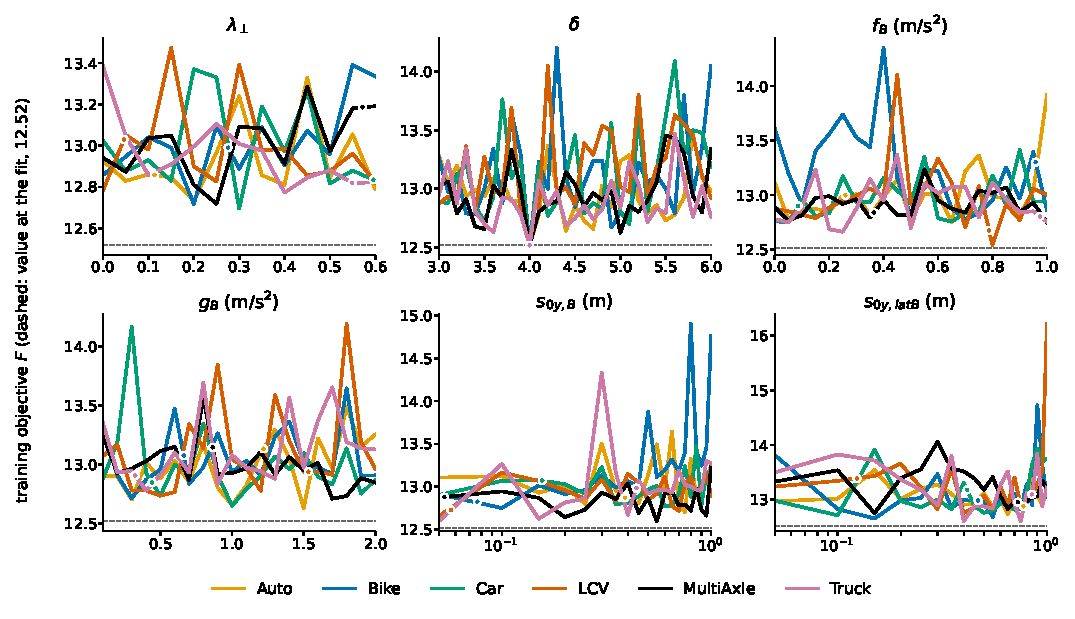
\includegraphics[width=\textwidth]{fig_oat_weak.pdf}
\caption{Profiles as in Figure~\ref{fig:key}, for six parameters that the data
hardly constrain: the lateral anisotropy, the IDM exponent and the four
road-edge parameters. Note the narrow range of the vertical axes.}
\label{fig:weak}
\end{figure}

\begin{figure}[H]\centering
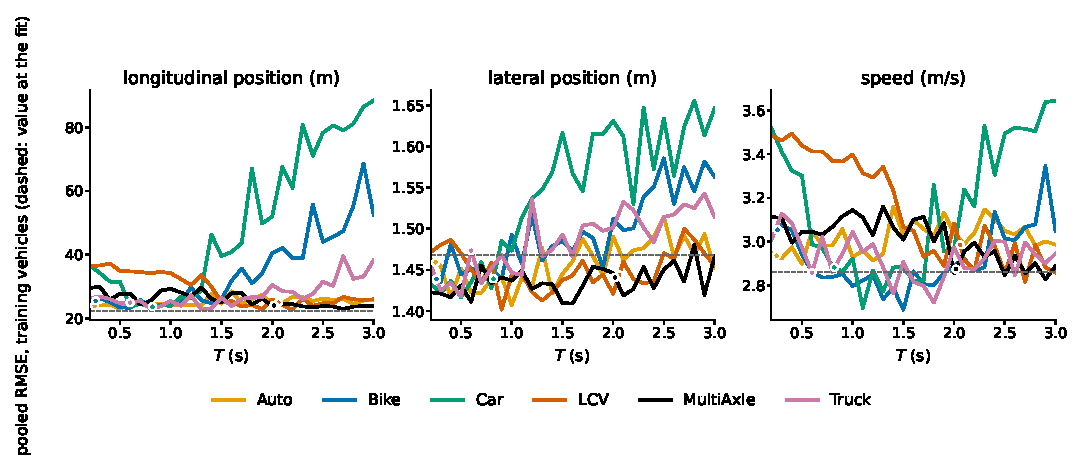
\includegraphics[width=\textwidth]{fig_oat_T_rmse.pdf}
\caption{Pooled RMSE of the training vehicles against the time gap $T$ of each
class, all other parameters at the fit: longitudinal position, lateral position
and speed. Dashed: value at the fit.}
\label{fig:Trmse}
\end{figure}

\paragraph{Observations.}
\begin{itemize}\setlength{\itemsep}{1pt}
\item Almost every point of every profile lies above the fitted $F$ (the lowest
point is on median 0.20 above it, at most 0.54): the \key{fit sits in a narrow
dip} of the rough objective, and moving any one parameter by a single
granularity step raises $F$ by a few tenths.
\item The \key{car-following parameters of the largest classes matter most}:
over its box, $T$ changes $F$ by 26.8 for Car and 19.6 for Bike, $s_0$ by 20.9
and 17.0, $a$ by 14.3 for Car and $b$ by 12.7 for LCV.
\item Of the lateral parameters, $s_{0y}$ for Bike (25.6), $\sigma$ for
Bike (9.3) and $\tau$ for Car (8.4) matter.
\item \key{Hardly constrained by the data}: the lateral anisotropy $\lambda_\perp$
(range 0.5--0.7), the road-edge parameters $f_B$, $g_B$ and $s_{0y,B}$ (mostly
below 1.7), the exponent $\delta$ (0.9--1.7), and most parameters of Auto and
MultiAxle, the classes with the fewest training vehicles (22 and 13).
\item The pooled RMSEs do not always move with $F$: raising Bike's time gap
to 1.5\,s lowers the speed error from 2.86 to 2.69\,m/s
(Figure~\ref{fig:Trmse}) while $F$ rises from 12.52 to 15.0, and raising
Car's $b$ to 2.5\,m/s$^2$ gives 2.70\,m/s at $F=17.1$. $F$ weighs position,
lateral and speed errors together, and an improvement in one can cost more in
the others.
\item For Bike $v_0$ and $a$ and for Car $b$ the fitted value lies at the edge
of the box and $F$ rises away from it, so these boxes bind.
\end{itemize}
%======================================================================
\section{Results}
\label{sec:results}
All figures in this section are from the run with all parameters free.

\subsection{Space-time diagrams}
Figure~\ref{fig:allx} shows the position of every vehicle along the section
against time, measured and calibrated, and Figure~\ref{fig:ally} the lateral
position against time; the same diagrams for each class are in
Appendix~\ref{app:stclass}. Calibrated vehicles are below 0.5\,m/s on $24\,\%$
of frames, against $36\,\%$ measured.

\begin{figure}[H]\centering
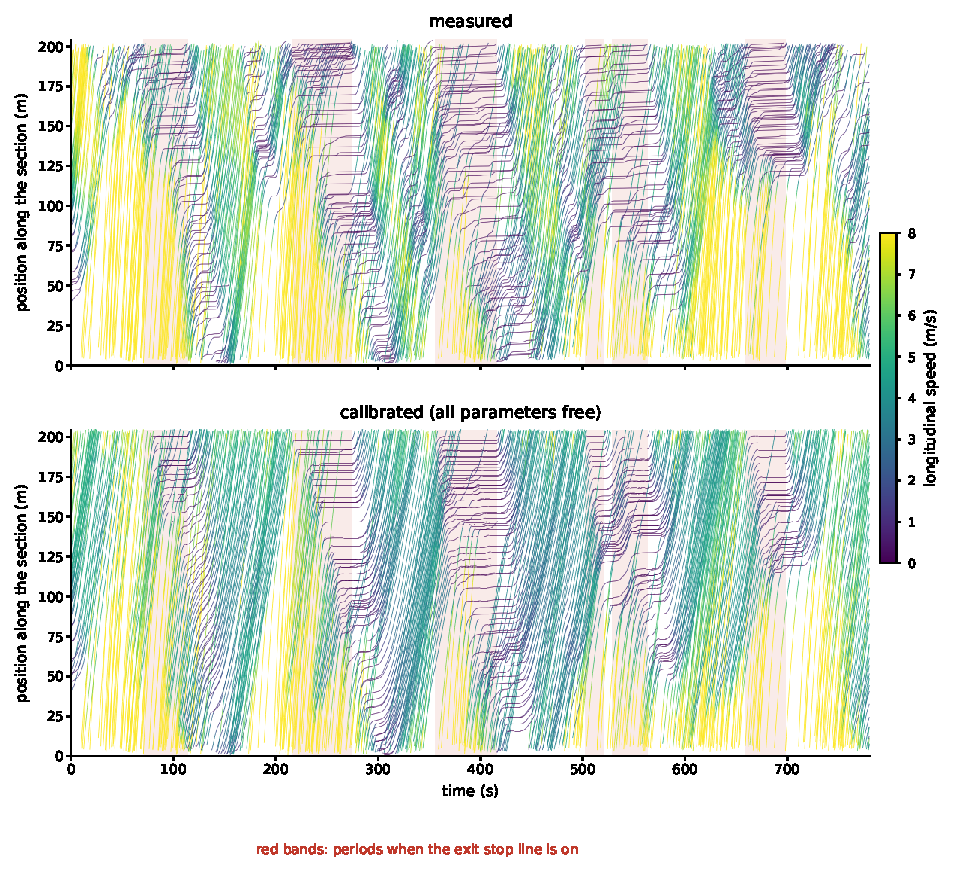
\includegraphics[width=\textwidth,height=0.75\textheight,keepaspectratio]{fig_all_x.pdf}
\caption{Space-time diagram of all 554 vehicles over the whole record: position
along the section against time, coloured by longitudinal speed. Top: measured.
Bottom: calibrated, one simulation of the whole record. Red bands: periods when
the exit stop line is on.}
\label{fig:allx}
\end{figure}

\paragraph{Observations.}
\begin{itemize}\setlength{\itemsep}{1pt}
\item \key{Queues form at the measured times}, growing back from the exit during
each stop, for every class except Bike (Figure~\ref{fig:stx}).
\item The calibrated queues are \key{shallower and shorter} than the measured
ones.
\item Between queues the calibrated vehicles travel at a \key{more uniform
speed}: the fast segments of the measured traffic near the entry, visible in
yellow, are largely missing.
\end{itemize}

\begin{figure}[H]\centering
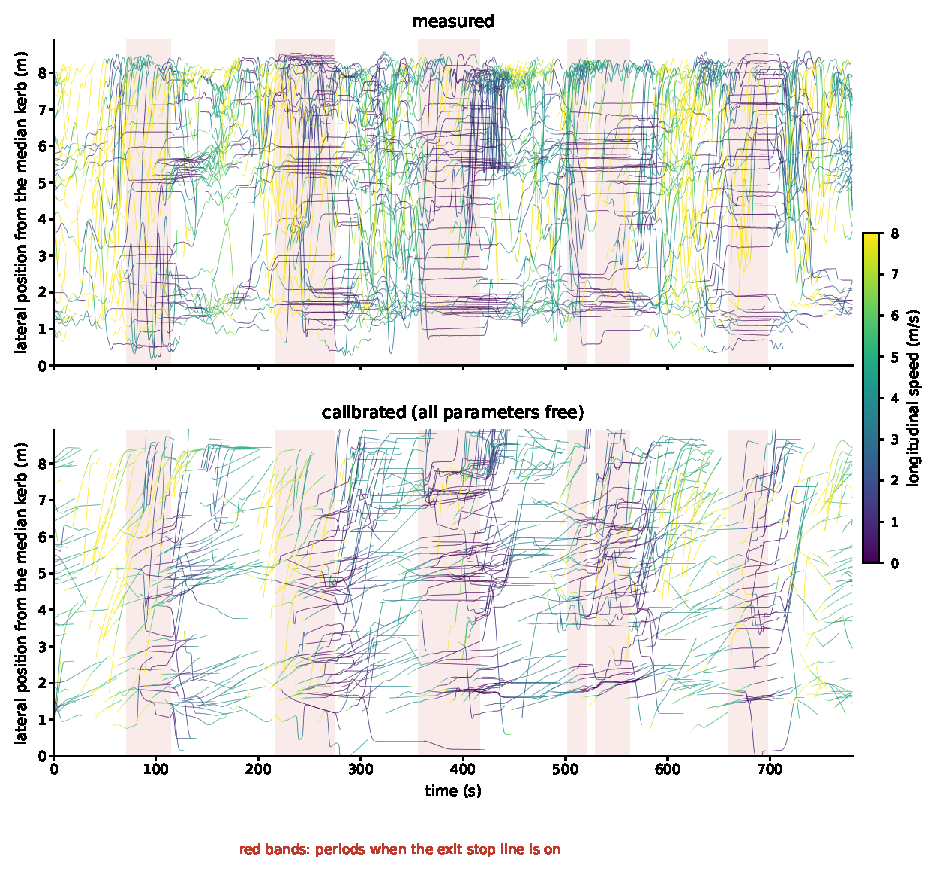
\includegraphics[width=\textwidth,height=0.75\textheight,keepaspectratio]{fig_all_y.pdf}
\caption{Lateral position of all vehicles against time, measured (top) and
calibrated (bottom), coloured by longitudinal speed; $y=0$ is the median kerb
and $y=8.9$\,m the far edge.}
\label{fig:ally}
\end{figure}

\paragraph{Observations.}
\begin{itemize}\setlength{\itemsep}{1pt}
\item Measured vehicles, Cars, LCVs and Trucks in particular
(Figure~\ref{fig:sty}), hold a lateral position for long periods and then
\key{move sideways in a few seconds}, which shows as steps.
\item Calibrated vehicles instead \key{drift slowly and steadily}, as slanted
lines, and make few abrupt moves.
\item Calibrated Bikes gather towards the far edge ($y\approx8$\,m) more
than measured ones.
\item This matches the model structure: with \key{no lateral target}, lateral
motion can only be a reaction to neighbours and edges followed by decay
(Section~\ref{sec:model}).
\end{itemize}

\subsection{Plan view of single vehicles}
Figure~\ref{fig:xy} shows the path of single held-out vehicles seen from above.
For each class the two held-out vehicles with the lowest $F$ are on the left and
the two with the highest $F$ on the right (among vehicles present for at least
10\,s and travelling at least 60\,m; Trailer has two held-out vehicles, one on
each side).

\begin{figure}[H]\centering
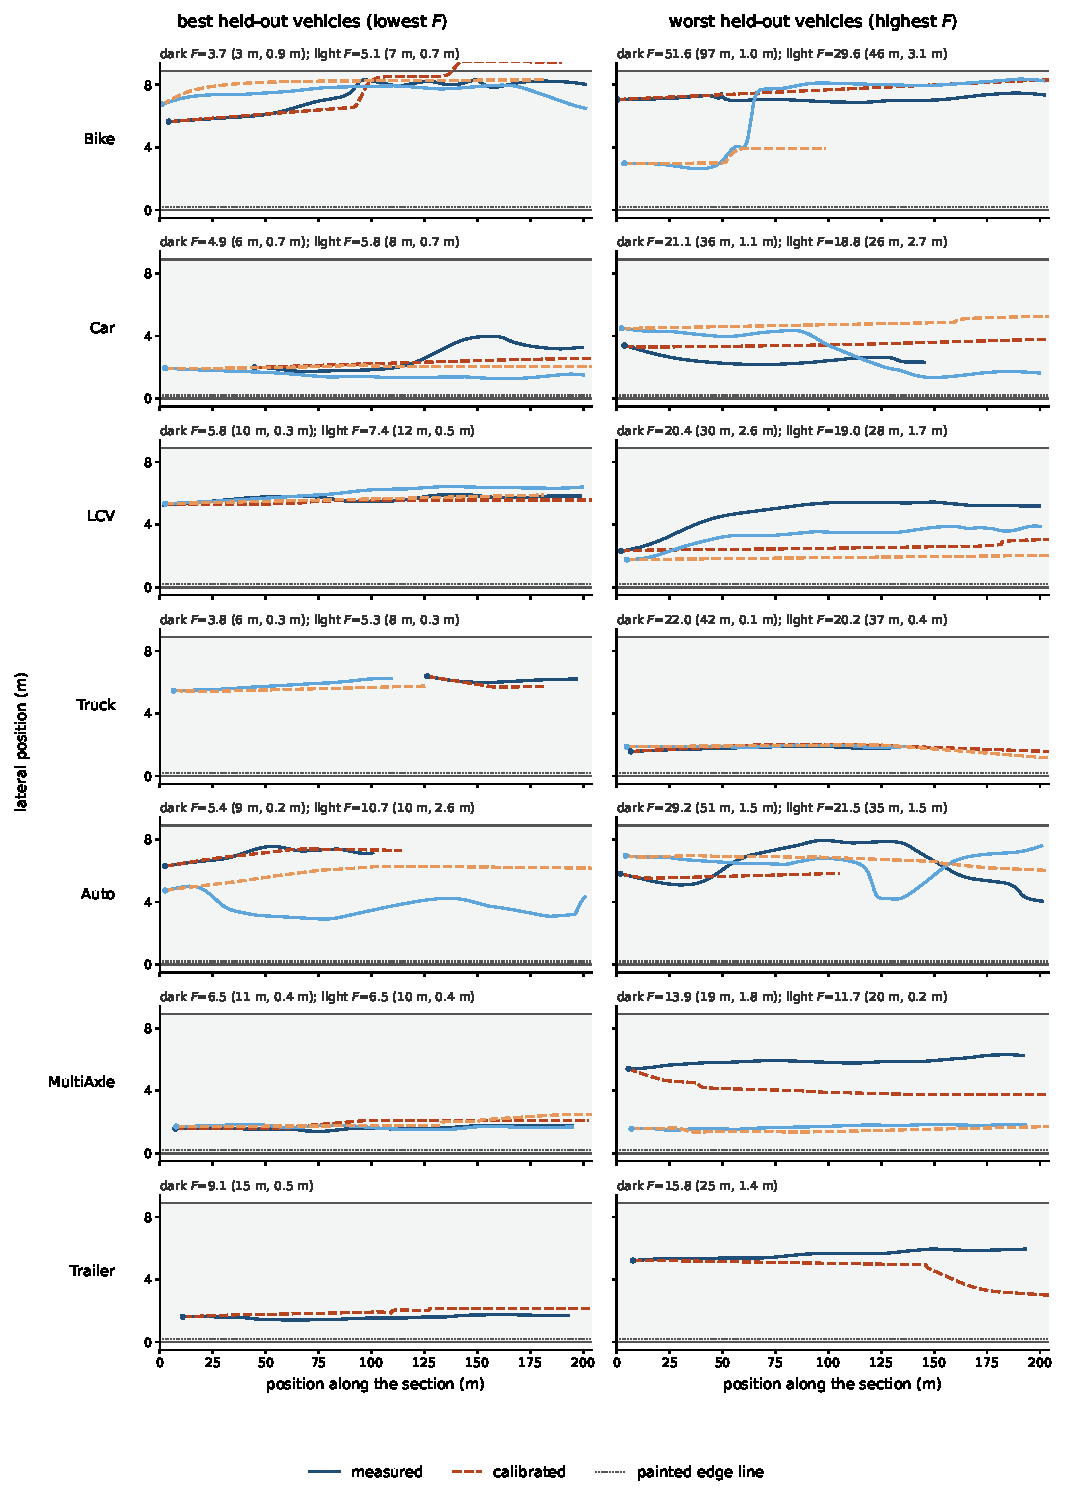
\includegraphics[width=\textwidth,height=0.85\textheight,keepaspectratio]{fig_xy.pdf}
\caption{Lateral against longitudinal position of held-out vehicles, measured
(solid) and calibrated (dashed). Left: the two vehicles of the class with the
lowest $F$; right: the two with the highest. The first vehicle is drawn dark,
the second light; panel titles give $F$, longitudinal RMSE and lateral RMSE of
each. Dot: entry point. The lateral axis is stretched about twenty-fold.}
\label{fig:xy}
\end{figure}

\paragraph{Observations.}
\begin{itemize}\setlength{\itemsep}{1pt}
\item The \key{best vehicles keep close to their measured paths}, with
longitudinal RMSE of 3--15\,m and lateral RMSE below 1\,m.
\item The worst fail \key{laterally}: the measured vehicle makes a deliberate
move across the road (for example a Bike from $y\approx3$ to 8\,m, or a
MultiAxle that the model moves the other way) that the calibrated vehicle does
not make.
\item They also fail \key{longitudinally}: the calibrated vehicle falls out of
step with its measured twin, typically by joining or leaving a queue at a
different time, which gives errors of 30--100\,m.
\end{itemize}

\subsection{Speed distributions}
\begin{figure}[H]\centering
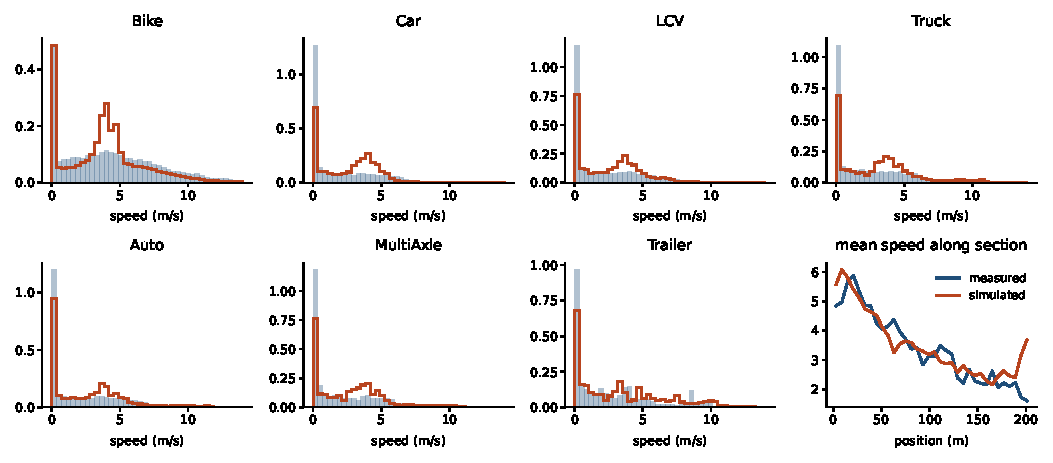
\includegraphics[width=\textwidth]{fig_classspeed.pdf}
\caption{Distribution of longitudinal speed per class over all frames of all
vehicles, measured (filled) and calibrated (line); vertical axis: probability
density. Last panel: mean speed against position along the section.}
\label{fig:speed}
\end{figure}

\paragraph{Observations.}
\begin{itemize}\setlength{\itemsep}{1pt}
\item For every class the calibrated speeds have a \key{peak around 4\,m/s}
that the measured ones do not; the measured speeds spread more evenly between
0 and 10\,m/s.
\item The share of stopped frames is matched for Bike and is \key{too low
for all other classes}, in line with the shallower queues of Figure~\ref{fig:stx}.
\item Mean speed along the section \key{follows the measured decline} from about
6\,m/s at the entry to about 2\,m/s near the exit, except in the last 10\,m,
where calibrated vehicles speed up again as they leave.
\end{itemize}

\subsection{Spread of errors between vehicles}
The pooled RMSE of Table~\ref{tab:runs} is one number per set of vehicles.
Figure~\ref{fig:rmsesd} and Table~\ref{tab:rmsesd} show how the error of
single vehicles varies within each class: each vehicle's own RMSE over the
frames on which it is scored.

\begin{figure}[H]\centering
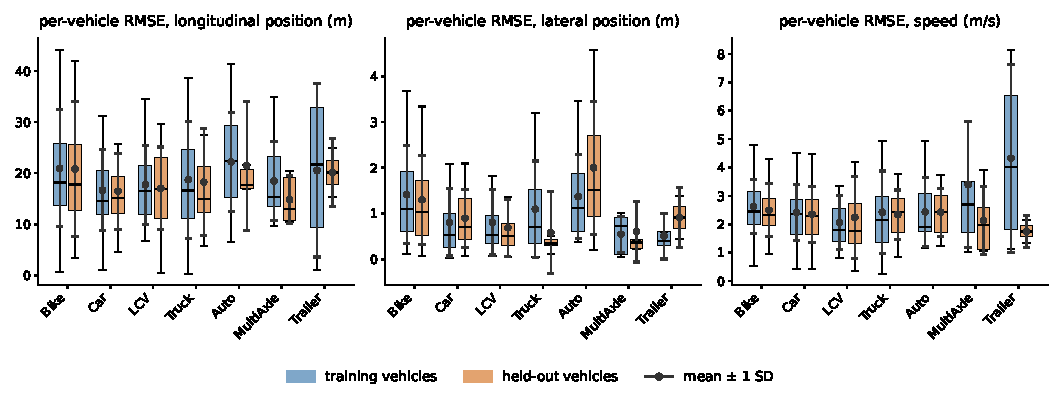
\includegraphics[width=\textwidth]{fig_rmse_spread.pdf}
\caption{Per-vehicle RMSE by class, training and held-out vehicles (box:
quartiles; whiskers: 1.5 times the interquartile range, outliers not drawn;
point and bar: mean and one standard deviation).}
\label{fig:rmsesd}
\end{figure}

\begin{table}[H]\centering\footnotesize
\caption{Mean (standard deviation) of the per-vehicle RMSE by class.}
\label{tab:rmsesd}
\begin{tabular}{@{}l lll lll@{}}\toprule
 & \multicolumn{3}{c}{training} & \multicolumn{3}{c}{held out}\\
\cmidrule(lr){2-4}\cmidrule(l){5-7}
class & long.\ (m) & lat.\ (m) & speed (m/s) & long.\ (m) & lat.\ (m) & speed (m/s)\\\midrule
Bike & 20.9 (11.5) & 1.41 (1.07) & 2.62 (0.94) & 20.8 (13.2) & 1.30 (0.97) & 2.49 (0.94)\\
Car & 16.7 (7.9) & 0.81 (0.74) & 2.41 (0.99) & 16.4 (7.4) & 0.90 (0.63) & 2.35 (0.99)\\
LCV & 17.7 (7.7) & 0.81 (0.72) & 2.06 (0.95) & 17.0 (8.1) & 0.69 (0.62) & 2.24 (1.43)\\
Truck & 18.7 (11.5) & 1.10 (1.05) & 2.43 (1.45) & 18.2 (10.4) & 0.58 (0.90) & 2.34 (0.87)\\
Auto & 22.2 (9.6) & 1.37 (0.93) & 2.44 (1.20) & 21.4 (12.6) & 2.00 (1.45) & 2.43 (0.84)\\
MultiAxle & 18.5 (7.8) & 0.55 (0.40) & 3.40 (2.22) & 14.8 (4.7) & 0.61 (0.67) & 2.13 (1.19)\\
Trailer & 20.5 (17.0) & 0.51 (0.50) & 4.32 (3.30) & 20.1 (6.7) & 0.92 (0.66) & 1.75 (0.55)\\
\bottomrule\end{tabular}

\end{table}

\paragraph{Observations.}
\begin{itemize}\setlength{\itemsep}{1pt}
\item The \key{spread between vehicles of the same class is large}: the standard
deviation of the per-vehicle longitudinal RMSE is about half its mean (for Bike,
20.9\,m with a standard deviation of 11.5\,m).
\item \key{Auto and Bike} have the largest lateral errors and the widest lateral
spread.
\item Training and held-out vehicles have \key{similar distributions} in every
class; the larger speed errors of the few training MultiAxle and Trailer
vehicles come from a handful of vehicles.
\end{itemize}

\subsection{Errors over time}
Figure~\ref{fig:rmsetime} shows when the errors arise. The top row bins the
error by time since each vehicle entered the section, which shows whether it
grows the longer a vehicle is simulated from its single entry state. The bottom
row bins it by time in the record, which shows whether particular periods, such
as the stop phases, are reproduced worse than others.

\begin{figure}[H]\centering
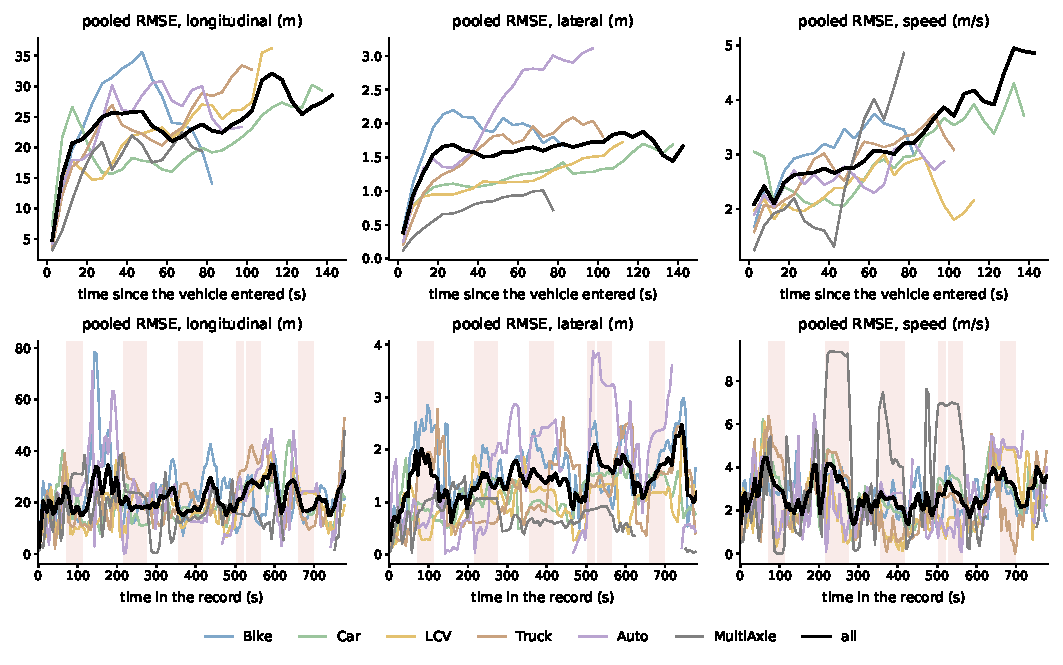
\includegraphics[width=\textwidth]{fig_rmse_time.pdf}
\caption{Pooled RMSE in 5\,s bins over all scored vehicles, per class (thin)
and overall (thick). Top: against time since the vehicle entered, bins with at
least ten vehicles. Bottom: against time in the record; red bands: periods when
the exit stop line is on. Trailer is included in ``all'' only.}
\label{fig:rmsetime}
\end{figure}

\paragraph{Observations.}
\begin{itemize}\setlength{\itemsep}{1pt}
\item The position errors grow during the first 20--30\,s after a vehicle
enters and then \key{level off}, at about 20--25\,m along the road and
1.5--1.8\,m across it, so they do not keep compounding over a vehicle's time on
the section.
\item The \key{speed error keeps rising} with time since entry, but the late bins
contain only the vehicles that stay longest, which are those held in queues.
\item Over the record, the \key{errors are highest around the stop phases}, when
the timing of queuing and release matters most, and lowest in between.
\end{itemize}

%======================================================================
\section{Conclusions}
\label{sec:concl}
\begin{enumerate}\setlength{\itemsep}{2pt}
\item The IAM was calibrated to a 781\,s record of lane-free mixed traffic by
simulating all 554 vehicles together from their entry states, with one
parameter vector per class and an exit stop line taken from the measured stops.
With all parameters free, held-out vehicles are predicted over their whole time
on the section with pooled errors of 22.4\,m along the road, 1.51\,m across it
and 2.60\,m/s in speed, as well as training vehicles.
\item IDM values calibrated elsewhere on leader-follower pairs do not transfer
to this site. Fixing them raises the held-out longitudinal error to 35.5\,m
(single set) and 49.3\,m (per class), mainly because their desired speeds are
far above the speeds on this congested stretch.
\item The fit is governed by a few parameters, chiefly the time gap, minimum
gap, acceleration and deceleration of Bike, Car and LCV and the lateral widths
of Bike. The lateral anisotropy, the road-edge parameters and the IDM exponent
are hardly constrained by these data, and several fitted values sit at their
bounds.
\item The calibrated traffic reproduces when and where queues form and the
fall of speed along the section, but it queues less than measured traffic, its
speeds cluster too narrowly around 4\,m/s, and its lateral motion is a slow
drift rather than the discrete sideways moves of real vehicles. The last point
follows from the model, which has no lateral target.
\item Position errors build up in the first 20--30\,s after entry and then
level off; the largest errors occur around the stop phases.
\end{enumerate}

\section{Future work}
\label{sec:future}
\begin{enumerate}\setlength{\itemsep}{2pt}
\item Add a lateral target to the model, such as a preferred lateral position or
a choice of gap, so that vehicles can make deliberate sideways moves, and model
how Bikes pass the stop line and filter through queues.
\item Model differences between drivers of one class, which a single vector
per class averages out: in \cite{duggal} the spread of IDM values between
drivers is about as large as their mean, and here per-vehicle errors vary
widely within each class (Table~\ref{tab:rmsesd}). Two steps: a hierarchical
calibration, in which each vehicle's IDM parameters are drawn from a class
distribution whose mean and spread are fitted; and a regression that predicts a
vehicle's parameters from its first 5--10\,s in the data (mean speed, peak
acceleration, smallest accepted gap, lateral moves), trained on per-vehicle fits
and scored only on the rest of each trajectory.
\item Fix the parameters that the data do not constrain (lateral anisotropy,
road-edge parameters, $\delta$) and refit the rest, with several optimiser seeds,
and reopen the boxes that bind (Bike $v_0$ and $a$, Car $b$, Car and LCV $\sigma$).
\item Extend the sensitivity analysis to variance-based indices \cite{punzo},
which capture interactions between parameters, and use the CMA-ES covariance
to identify parameters that trade off against each other.
\item Validate on another period or site, since the split by vehicle within one
record measures transfer within the same traffic only.
\item Compare the calibrated IAM with data-driven approaches on the same record,
the second direction set out in the Introduction.
\end{enumerate}

%======================================================================
\section*{Acknowledgements}
\addcontentsline{toc}{section}{Acknowledgements}
I thank Prof.\ Bhargava Rama Chilukuri, Department of Civil Engineering, IIT
Madras, for his guidance throughout this work. I also thank Suhaib Nazir,
Research Scholar, TR Division, Civil Engineering Department, for providing the
trajectory dataset and the vehicle dimensions, and Dr.\ Chandrashekar C,
Postdoctoral Researcher, Department of Civil Engineering, IIT Madras, for
providing the IDM parameter values and the presentation on the IDM calibration
work on which the fixed-IDM runs are based.
%======================================================================
\begin{thebibliography}{99}
\bibitem{lw55} M.~J.~Lighthill and G.~B.~Whitham, ``On kinematic waves. II. A
theory of traffic flow on long crowded roads,'' \emph{Proceedings of the Royal
Society A}, 229(1178):317--345, 1955.
\bibitem{richards56} P.~I.~Richards, ``Shock waves on the highway,''
\emph{Operations Research}, 4(1):42--51, 1956.
\bibitem{ph71} I.~Prigogine and R.~Herman, \emph{Kinetic Theory of Vehicular
Traffic}, Elsevier, New York, 1971.
\bibitem{gipps81} P.~G.~Gipps, ``A behavioural car-following model for computer
simulation,'' \emph{Transportation Research Part B}, 15(2):105--111, 1981.
\bibitem{papageorgiou21} M.~Papageorgiou, K.-S.~Mountakis, I.~Karafyllis,
I.~Papamichail and Y.~Wang, ``Lane-free artificial-fluid concept for vehicular
traffic,'' \emph{Proceedings of the IEEE}, 109(2):114--121, 2021.
\bibitem{vo98} P.~Fiorini and Z.~Shiller, ``Motion planning in dynamic
environments using velocity obstacles,'' \emph{International Journal of Robotics
Research}, 17(7):760--772, 1998.
\bibitem{rvo08} J.~van den Berg, M.~Lin and D.~Manocha, ``Reciprocal velocity
obstacles for real-time multi-agent navigation,'' \emph{IEEE International
Conference on Robotics and Automation}, 2008.
\bibitem{orca11} J.~van den Berg, S.~J.~Guy, M.~Lin and D.~Manocha, ``Reciprocal
n-body collision avoidance,'' in \emph{Robotics Research}, Springer Tracts in
Advanced Robotics 70, 3--19, 2011.
\bibitem{simtram15} T.~V.~Mathew, C.~R.~Munigety and A.~Bajpai, ``Strip-based
approach for the simulation of mixed traffic conditions,'' \emph{Journal of
Computing in Civil Engineering}, 29(5):04014069, 2015.
\bibitem{hm95} D.~Helbing and P.~Moln\'ar, ``Social force model for pedestrian
dynamics,'' \emph{Physical Review E}, 51(5):4282--4286, 1995.
\bibitem{ns92} K.~Nagel and M.~Schreckenberg, ``A cellular automaton model for
freeway traffic,'' \emph{Journal de Physique I}, 2(12):2221--2229, 1992.
\bibitem{mallikarjuna09} C.~Mallikarjuna and K.~R.~Rao, ``Cellular automata
model for heterogeneous traffic,'' \emph{Journal of Advanced Transportation},
43(3):321--345, 2009.
\bibitem{robusttp19} R.~Chandra, U.~Bhattacharya, C.~Roncal, A.~Bera and
D.~Manocha, ``RobustTP: end-to-end trajectory prediction for heterogeneous
road-agents in dense traffic with noisy sensor inputs,'' \emph{ACM Computer
Science in Cars Symposium}, 2019.
\bibitem{gamma} Y.~Luo, P.~Cai, Y.~Lee and D.~Hsu, ``GAMMA: a general agent
motion model for autonomous driving,'' \emph{IEEE Robotics and Automation
Letters}, 2022; arXiv:1906.01566.
\bibitem{autorvo18} Y.~Ma, D.~Manocha and W.~Wang, ``AutoRVO: local navigation
with dynamic constraints in dense heterogeneous traffic,'' arXiv:1804.02915,
2018.
\bibitem{qin22} J.~Qin, S.~Ma, L.~Zhang, Q.~Wang and G.~Feng, ``Modeling and
simulation for non-motorized vehicle flow on road based on modified social
force model,'' \emph{Mathematics}, 11(1):170, 2022.
\bibitem{firl12} J.~Firl, H.~St\"ubing, S.~A.~Huss and C.~Stiller, ``Predictive
maneuver evaluation for enhancement of Car-to-X mobility data,'' \emph{IEEE
Intelligent Vehicles Symposium}, 558--564, 2012.
\bibitem{marvx13} J.~Firl, H.~St\"ubing, S.~A.~Huss and C.~Stiller, ``MARV-X:
applying maneuver assessment for reliable verification of Car-to-X mobility
data,'' \emph{IEEE Transactions on Intelligent Transportation Systems},
14(3):1301--1312, 2013.
\bibitem{traphic19} R.~Chandra, U.~Bhattacharya, A.~Bera and D.~Manocha,
``TraPHic: trajectory prediction in dense and heterogeneous traffic using
weighted interactions,'' \emph{IEEE/CVF Conference on Computer Vision and
Pattern Recognition}, 2019.
\bibitem{postnikov21} A.~Postnikov, A.~Gamayunov and G.~Ferrer, ``Transformer
based trajectory prediction,'' arXiv:2112.04350, 2021.
\bibitem{s2tnet21} W.~Chen, F.~Wang and H.~Sun, ``S2TNet: spatio-temporal
transformer networks for trajectory prediction in autonomous driving,''
\emph{Proceedings of the 13th Asian Conference on Machine Learning}, PMLR
157:454--469, 2021.
\bibitem{karalakou23} A.~Karalakou, D.~Troullinos, G.~Chalkiadakis and
M.~Papageorgiou, ``Deep reinforcement learning reward function design for
autonomous driving in lane-free traffic,'' \emph{Systems}, 11(3):134, 2023.
\bibitem{iam} M.~Treiber and A.~A.~Chaudhari, ``The intelligent-agent model: a
fully two-dimensional microscopic traffic flow model,'' arXiv:2310.16816, 2023;
accepted in \emph{Transportation Letters}.
\bibitem{pneuma20} E.~Barmpounakis and N.~Geroliminis, ``On the new era of urban
traffic monitoring with massive drone data: the pNEUMA large-scale field
experiment,'' \emph{Transportation Research Part C}, 111:50--71, 2020.
\bibitem{idm} M.~Treiber, A.~Hennecke and D.~Helbing, ``Congested traffic states
in empirical observations and microscopic simulations,'' \emph{Physical Review
E}, 62(2):1805--1824, 2000.
\bibitem{acc} A.~Kesting, M.~Treiber and D.~Helbing, ``Enhanced intelligent
driver model to access the impact of driving strategies on traffic capacity,''
\emph{Philosophical Transactions of the Royal Society A}, 368(1928):4585--4605,
2010.
\bibitem{cma} N.~Hansen, ``The CMA evolution strategy: a tutorial,''
arXiv:1604.00772, 2016.
\bibitem{pycma} N.~Hansen, Y.~Akimoto and P.~Baudis, ``CMA-ES/pycma on GitHub,''
Zenodo, doi:10.5281/zenodo.2559634, 2019.
\bibitem{duggal} N.~Duggal, ``Heterogeneity in vehicle following behaviour across
strict--staggered characteristics, LF pair type, and EV--non-EV interactions,''
project presentation (supervisors K.~K.~Srinivasan, B.~R.~Chilukuri and
O.~Okhrin), Department of Civil Engineering, IIT Madras, shared by
C.~Chandrashekar.
\bibitem{chandra} C.~Chandrashekar, calibrated IDM parameter values for mixed
traffic (table of parameters with common search bounds), personal communication,
Department of Civil Engineering, IIT Madras.
\bibitem{kt08} A.~Kesting and M.~Treiber, ``Calibrating car-following models by
using trajectory data: methodological study,'' \emph{Transportation Research
Record}, 2088:148--156, 2008.
\bibitem{kurtc16} V.~Kurtc and M.~Treiber, ``Calibrating the local and platoon
dynamics of car-following models on the reconstructed NGSIM data,'' in
\emph{Traffic and Granular Flow '15}, Springer, 2016; arXiv:1610.03124.
\bibitem{wosac23} N.~Montali et al., ``The Waymo Open Sim Agents Challenge,''
\emph{Advances in Neural Information Processing Systems (Datasets and
Benchmarks Track)}, 2023.
\bibitem{kipf17} T.~N.~Kipf and M.~Welling, ``Semi-supervised classification
with graph convolutional networks,'' \emph{International Conference on Learning
Representations}, 2017.
\bibitem{punzo} V.~Punzo, M.~Montanino and B.~Ciuffo, ``Do we really need to
calibrate all the parameters? Variance-based sensitivity analysis to simplify
microscopic traffic flow models,'' \emph{IEEE Transactions on Intelligent
Transportation Systems}, 16(1):184--193, 2015.
\end{thebibliography}

%======================================================================
\section*{Declaration of LLM use}
\addcontentsline{toc}{section}{Declaration of LLM use}
LLMs, namely Claude Sonnet 5.5 and Opus 5.5, were used for coding and formatting
purposes. The author owns the work and takes full responsibility for the
results reported.

%======================================================================
\appendix
\section{Origin of the fixed IDM values}
\label{app:idm}

\paragraph{Single set.} A single calibrated IDM parameter set \cite{chandra}:
$v_0=18.7615$\,m/s, $T=0.8899$\,s, $s_0=1.05$\,m, $a=2.0$\,m/s$^2$,
$b=2.6327$\,m/s$^2$, $\delta=4.42$. It is one set for all vehicle classes, and
it was calibrated for the plain IDM, whereas the car-following core here is ACC
(IDM blended with CAH), so the values do not transfer exactly. Its $s_0$, $a$
and $\delta$ equal the means of the variable-boundary IDM calibration in
\cite[slide~23]{duggal}, while its $v_0$, $T$ and $b$ differ.

\paragraph{Per class.} The study in \cite{duggal} calibrates the IDM on
leader-follower pairs from a different site (Indira Nagar, Chennai; pairs
identified within 30\,m longitudinally and 3\,m laterally,
\cite[slide~7]{duggal}), once per pair (pairwise) and once per group of pairs
(groupwise). We use the pairwise means by follower type \cite[slide~10]{duggal}
(Table~\ref{tab:duggal}). Several limitations bear on their use here:
\begin{itemize}\setlength{\itemsep}{1pt}
\item Only Auto, Bike, Car and EV followers are calibrated. LCV, Truck and Bus
followers occur in small numbers in the pair counts \cite[slide~8]{duggal} and
are not calibrated, and MultiAxle and Trailer do not appear.
\item The spread between pairs is about as large as the mean: for example
$v_0=21.3\pm6.8$\,m/s, $s_0=1.04\pm1.51$\,m and $b=1.28\pm1.46$\,m/s$^2$ for
Bike followers. The class means therefore differ little from each other.
\item In the groupwise calibration \cite[slide~10]{duggal} most values lie on a
bound of the search:
$v_0=29.6$ for Bike (cap 30), $s_0=0.40$--$0.44$ and $b=0.50$--$0.61$ for all
classes, and $\delta=3.00$ or $6.00$ for Auto, Bike and Car. These values reflect
the search box more than the drivers.
\item Time gaps are short ($T\approx0.25$--$0.31$\,s), as is usual for pair
calibration of closely staggered followers.
\item It is a single-leader, one-dimensional calibration with no lateral model,
so it gives nothing for the IAM parameters. The study's preferred model is
FVDM \cite[slides~23--24]{duggal}, whose parameters are reported by pair type and
do not apply to the IDM.
\end{itemize}

\begin{table}[H]\centering\footnotesize
\caption{IDM values used in the run ``Fixed IDM, per class''; pairwise means
from \cite[slide~10]{duggal}.}
\label{tab:duggal}
\begin{tabular}{@{}lrrrrrrl@{}}
\toprule
class & $v_0$ (m/s) & $T$ (s) & $s_0$ (m) & $a$ (m/s$^2$) & $b$ (m/s$^2$) & $\delta$ & source\\
\midrule
Auto & 20.27 & 0.31 & 0.64 & 2.57 & 0.93 & 4.50 & pairwise mean \cite{duggal}\\
Bike & 21.28 & 0.25 & 1.04 & 1.86 & 1.28 & 4.43 & pairwise mean \cite{duggal}\\
Car & 21.43 & 0.29 & 1.00 & 2.09 & 1.35 & 4.33 & pairwise mean \cite{duggal}\\
LCV & 20.0 & 0.31 & 1.10 & 1.90 & 1.12 & 4.33 & extrapolated from Car\\
Truck & 18.0 & 0.36 & 1.30 & 1.84 & 1.15 & 4.33 & extrapolated from Car\\
MultiAxle & 16.0 & 0.42 & 1.50 & 1.46 & 1.05 & 4.33 & extrapolated from Car\\
\bottomrule
\end{tabular}
\end{table}

\paragraph{Extrapolation to LCV, Truck and MultiAxle.} Starting from the Car
values of \cite{duggal}: $a$ and $b$ are scaled by each class's measured 95th percentile of
acceleration and of deceleration relative to Car in our record (acceleration
ratios 0.91, 0.88 and 0.70; deceleration ratios 0.83, 0.85 and 0.78); $v_0$ is
lowered with vehicle size (20, 18 and 16\,m/s), since the measured free-flow
speeds of all classes are about 8--9\,m/s on this congested stretch and give no
guidance; $T$ and $s_0$ are raised moderately with size within the short
time-gap regime of \cite{duggal}; and $\delta$ is kept at Car's value.

\paragraph{Free fit against the pairwise values.} Table~\ref{tab:duggalcmp}
compares the IDM values of the free fit with the pairwise means of
\cite[slide~10]{duggal}. The largest and most consistent difference is $v_0$,
lower by 1.1 (Auto) to 2.4 (Bike) standard deviations of the pairwise values,
in line with the low speeds of this record (median 2.1\,m/s, free-flow
85th percentile 8--13\,m/s).
\begin{table}[H]\centering\footnotesize
\caption{Free fit against the pairwise means of \cite[slide~10]{duggal}: fitted
value, pairwise mean, and their difference in standard deviations of the
pairwise values. $\delta$ is not calibrated in the free fit.}
\label{tab:duggalcmp}
\begin{tabular}{@{}llrrrrrr@{}}\toprule
class & & $v_0$ & $T$ & $s_0$ & $a$ & $b$ & $\delta$\\\midrule
Auto & free fit & 11.95 & 0.25 & 1.45 & 1.37 & 2.39 & 4.00\\
 & pairwise mean & 20.27 & 0.31 & 0.64 & 2.57 & 0.93 & 4.50\\
 & difference (SD) & -1.1 & -0.2 & +1.2 & -0.9 & +1.4 & -0.4\\
\midrule
Bike & free fit & 5.00 & 0.26 & 0.65 & 0.30 & 1.66 & 4.00\\
 & pairwise mean & 21.28 & 0.25 & 1.04 & 1.86 & 1.28 & 4.43\\
 & difference (SD) & -2.4 & +0.0 & -0.3 & -1.2 & +0.3 & -0.3\\
\midrule
Car & free fit & 5.65 & 0.82 & 0.30 & 1.56 & 0.50 & 4.00\\
 & pairwise mean & 21.43 & 0.29 & 1.00 & 2.09 & 1.35 & 4.33\\
 & difference (SD) & -2.3 & +1.7 & -0.5 & -0.4 & -0.5 & -0.3\\
\bottomrule\end{tabular}

\end{table}

\section{Space-time diagrams by class}
\label{app:stclass}
The diagrams of Figures~\ref{fig:allx} and~\ref{fig:ally}, drawn separately for
each vehicle class.

\begin{figure}[H]\centering
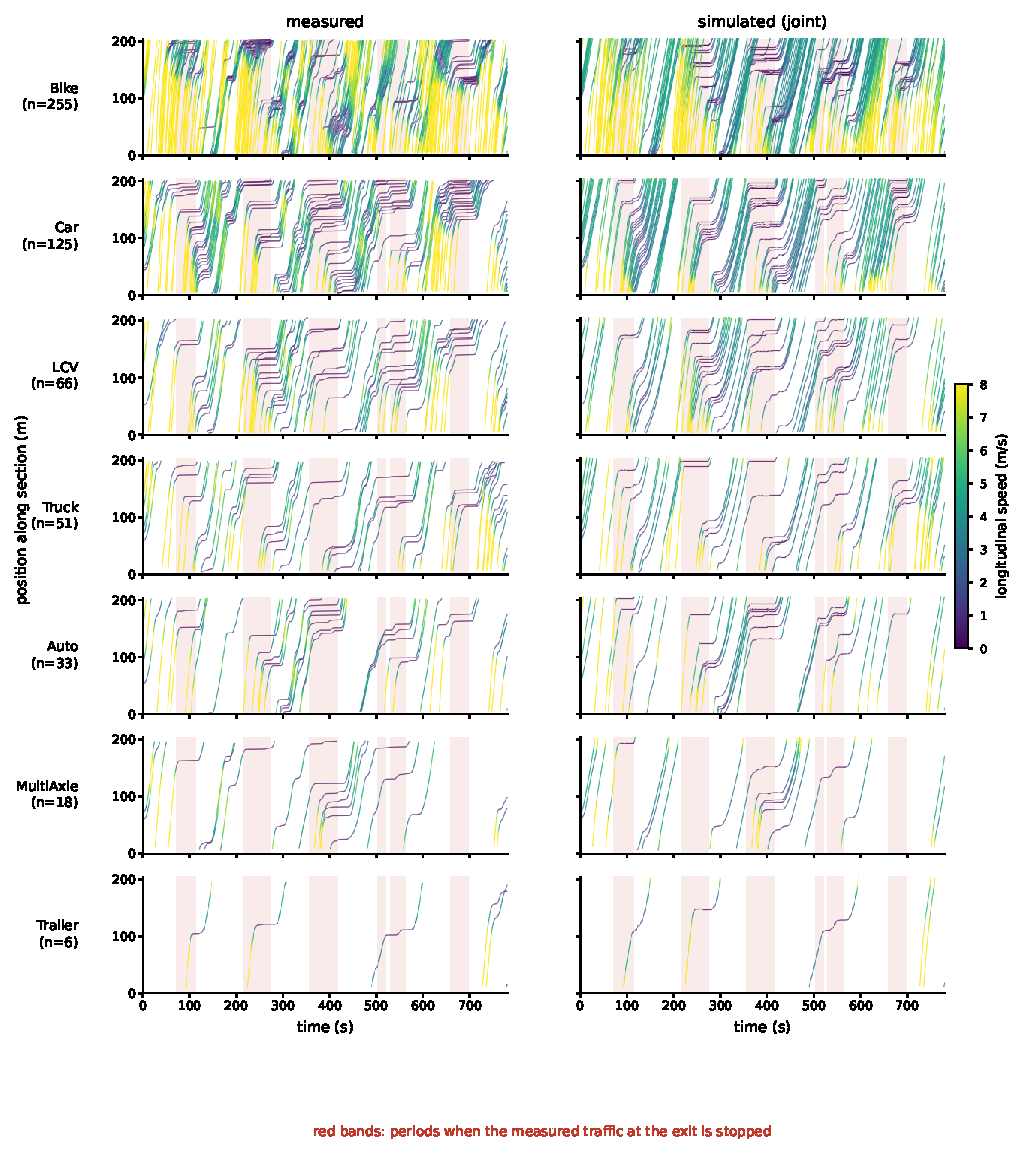
\includegraphics[width=\textwidth,height=0.8\textheight,keepaspectratio]{fig_st_x.pdf}
\caption{Space-time diagram per class over the whole record: position along
the section against time, coloured by longitudinal speed. Left: measured.
Right: calibrated, one simulation of the whole record. Red bands: periods when
the exit stop line is on. $n$: vehicles of the class.}
\label{fig:stx}
\end{figure}

\begin{figure}[H]\centering
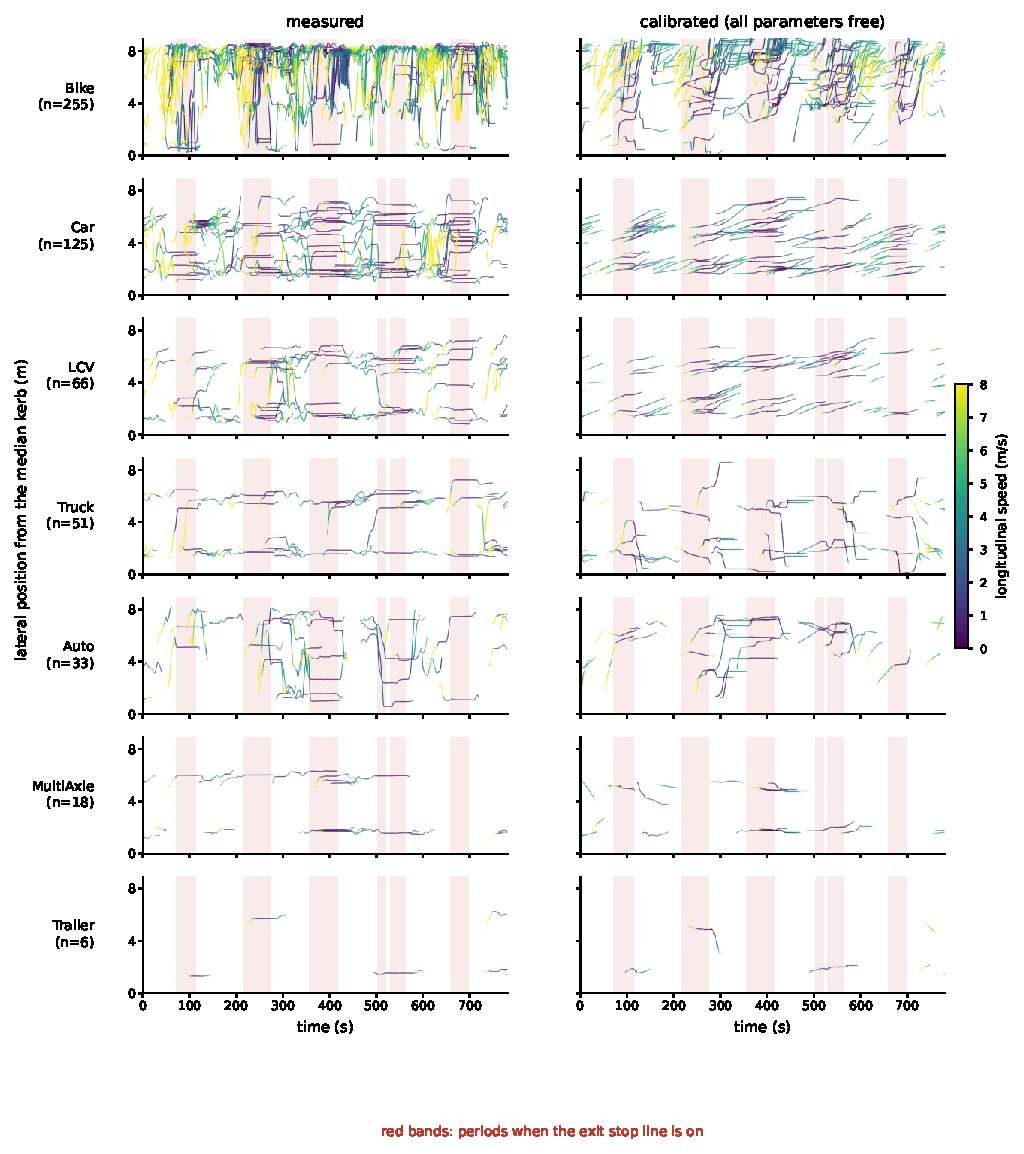
\includegraphics[width=\textwidth,height=0.8\textheight,keepaspectratio]{fig_st_y.pdf}
\caption{Lateral position against time per class, measured (left) and
calibrated (right), coloured by longitudinal speed; $y=0$ is the median kerb
and $y=8.9$\,m the far edge.}
\label{fig:sty}
\end{figure}

\section{Sensitivity profiles}
\label{app:prof}
The profiles of the one-at-a-time sensitivity analysis of the free fit
(Section~\ref{sec:calib}). Figure~\ref{fig:spread} summarises each profile by
the distribution of $F$ over all values tried: a tall box means the fit depends
strongly on that parameter; a box that stays on the dashed line means the data
hardly constrain it. Figures~\ref{fig:profF}--\ref{fig:profspeed} show all
profiles: training $F$ and the pooled RMSEs of the training vehicles against
the value of one parameter of one class, with all other parameters at the fit.

\begin{figure}[H]\centering
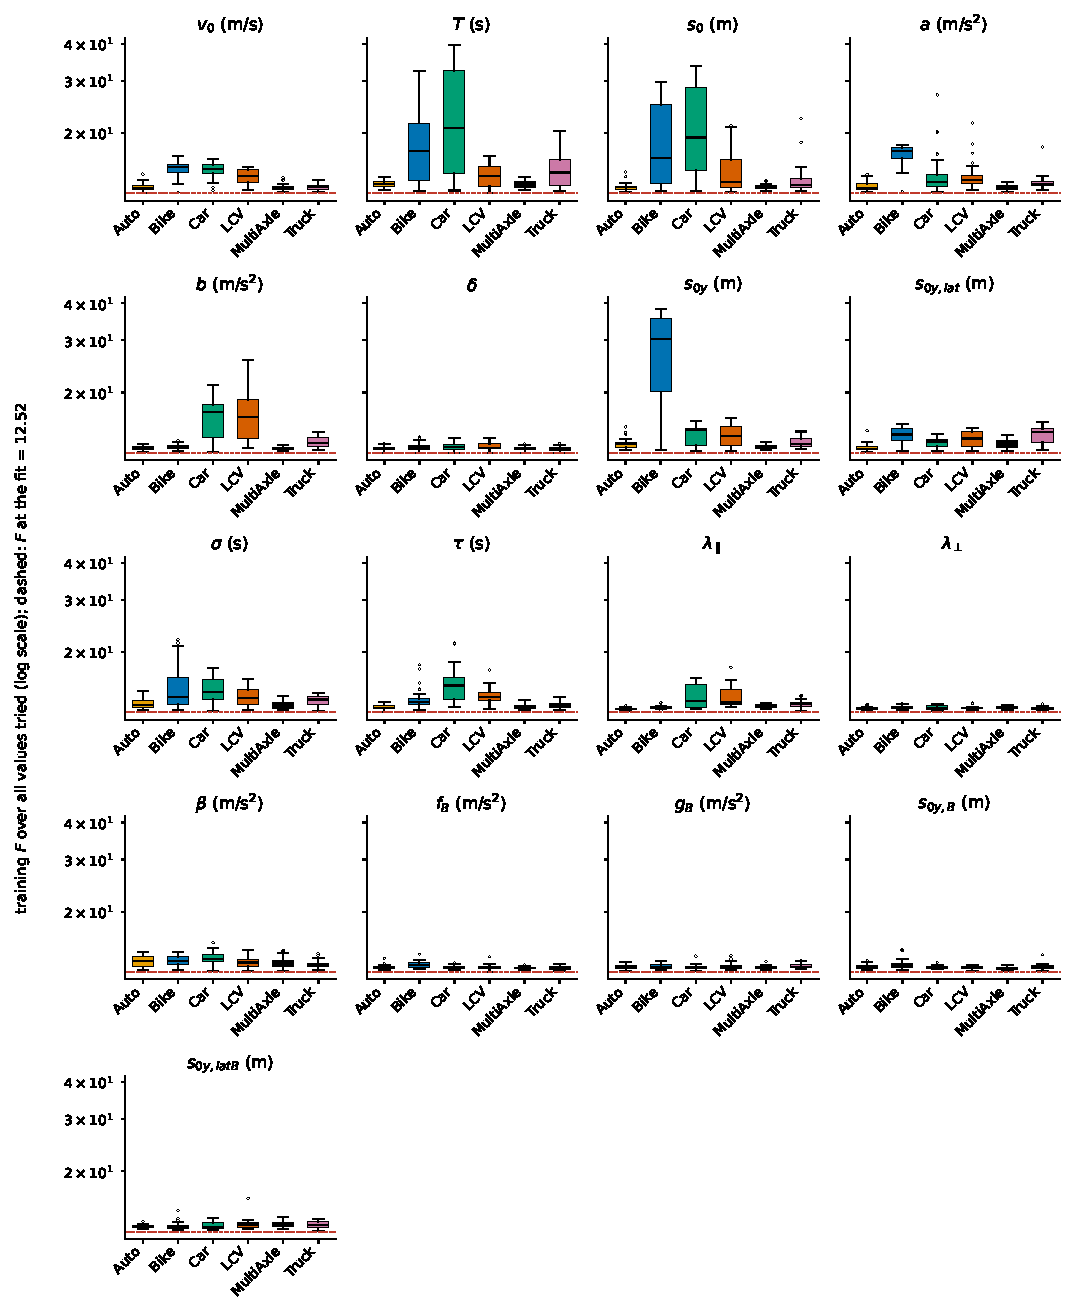
\includegraphics[width=\textwidth]{fig_oat_spread.pdf}
\caption{One-at-a-time sensitivity of the free fit: training objective $F$
over all values tried for each parameter, one box per class (box: quartiles;
whiskers: 1.5 times the interquartile range; points: outliers). Dashed line:
$F$ at the fit.}
\label{fig:spread}
\end{figure}

\begin{figure}[H]\centering
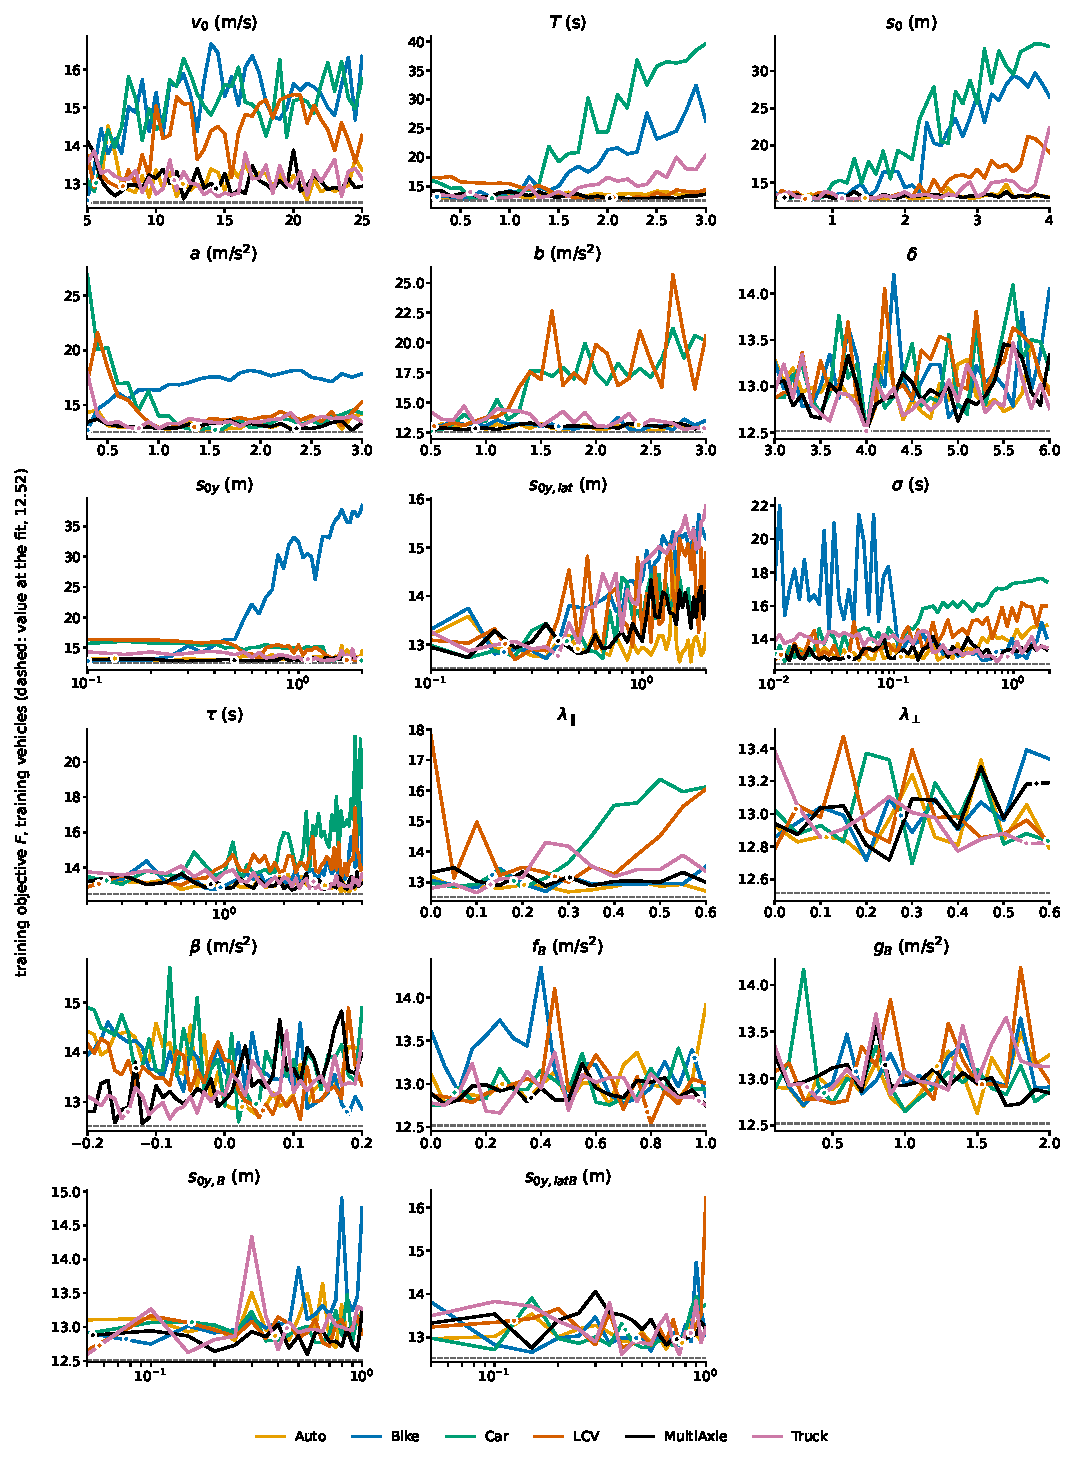
\includegraphics[width=\textwidth,height=0.85\textheight,keepaspectratio]{fig_oat_prof_F.pdf}
\caption{Profiles of the free fit: training objective $F$ against the value of
one parameter, one line per class, all other parameters at the fit. Dots:
fitted values (placed on the line between the two nearest grid points). Dashed:
$F$ at the fit. Log-scaled parameters are drawn on a log axis.}
\label{fig:profF}
\end{figure}

\begin{figure}[H]\centering
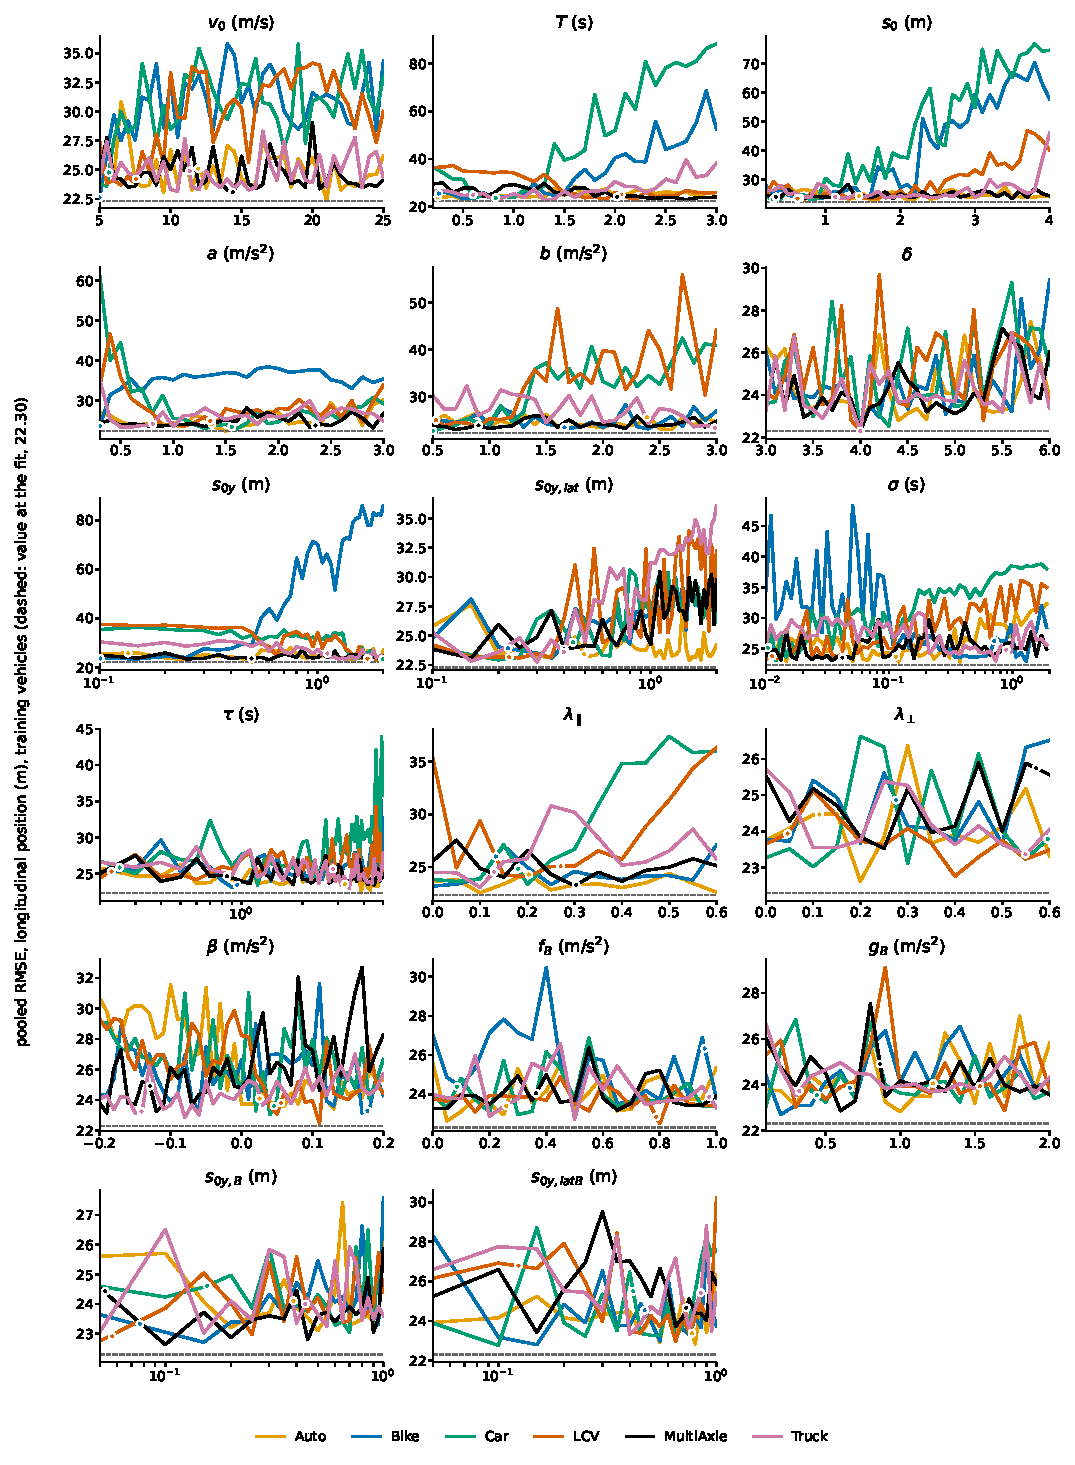
\includegraphics[width=\textwidth,height=0.85\textheight,keepaspectratio]{fig_oat_prof_long.pdf}
\caption{Profiles as in Figure~\ref{fig:profF}, for the pooled RMSE of
longitudinal position of the training vehicles.}
\label{fig:proflong}
\end{figure}

\begin{figure}[H]\centering
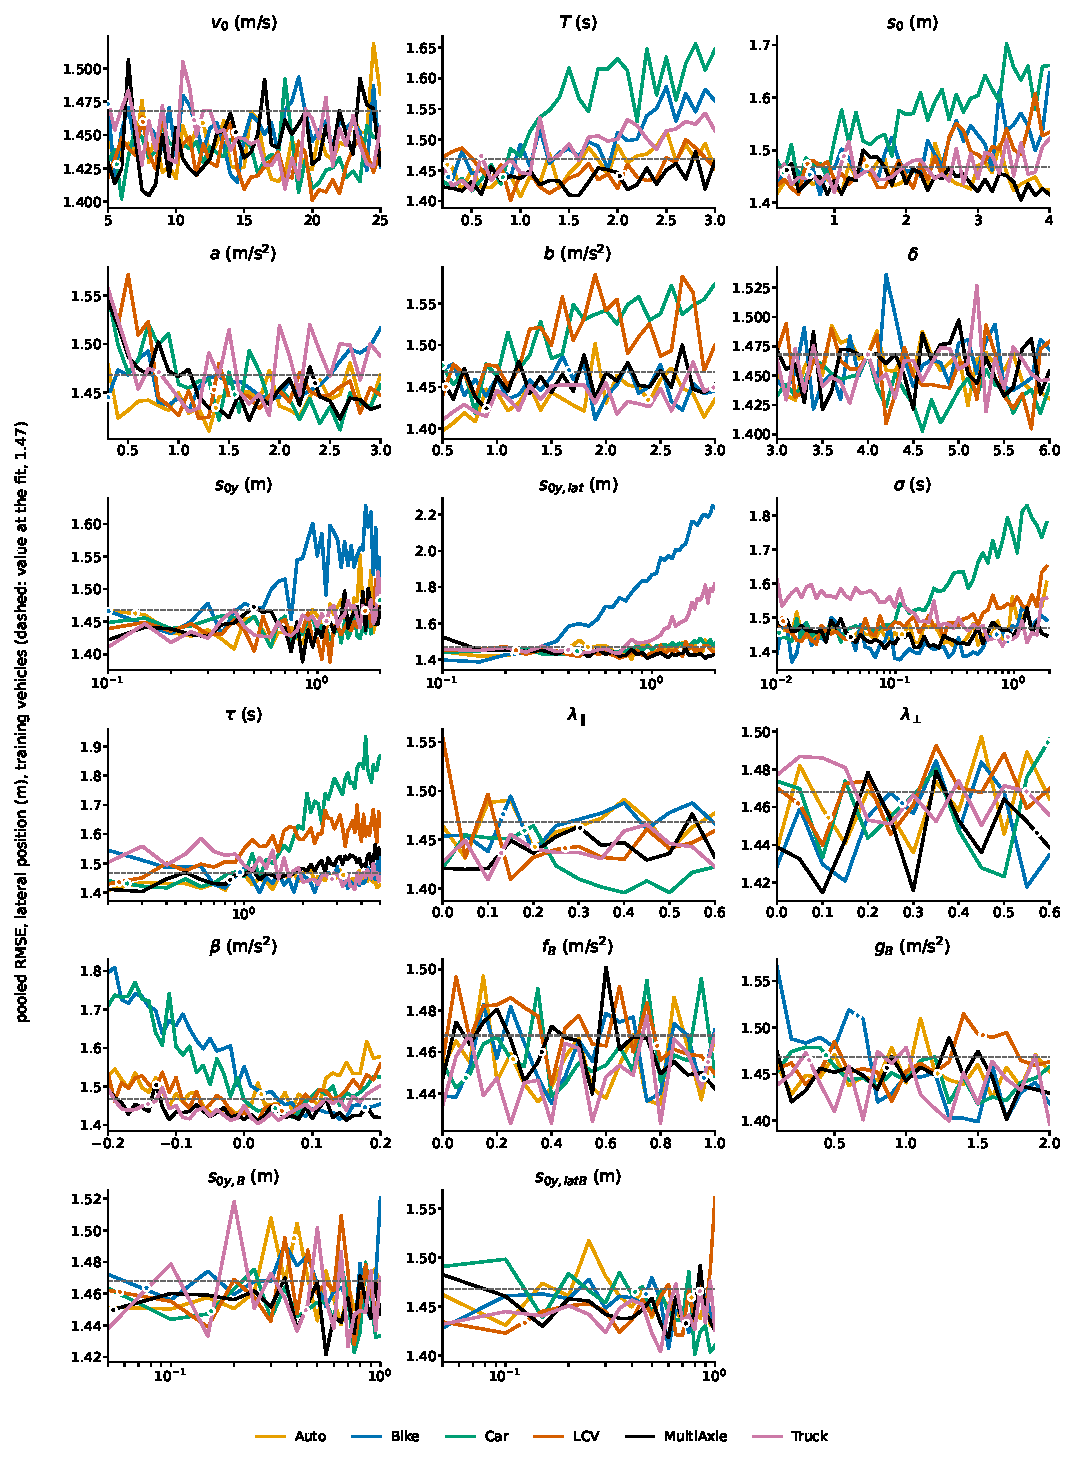
\includegraphics[width=\textwidth,height=0.85\textheight,keepaspectratio]{fig_oat_prof_lat.pdf}
\caption{Profiles as in Figure~\ref{fig:profF}, for the pooled RMSE of lateral
position of the training vehicles.}
\label{fig:proflat}
\end{figure}

\begin{figure}[H]\centering
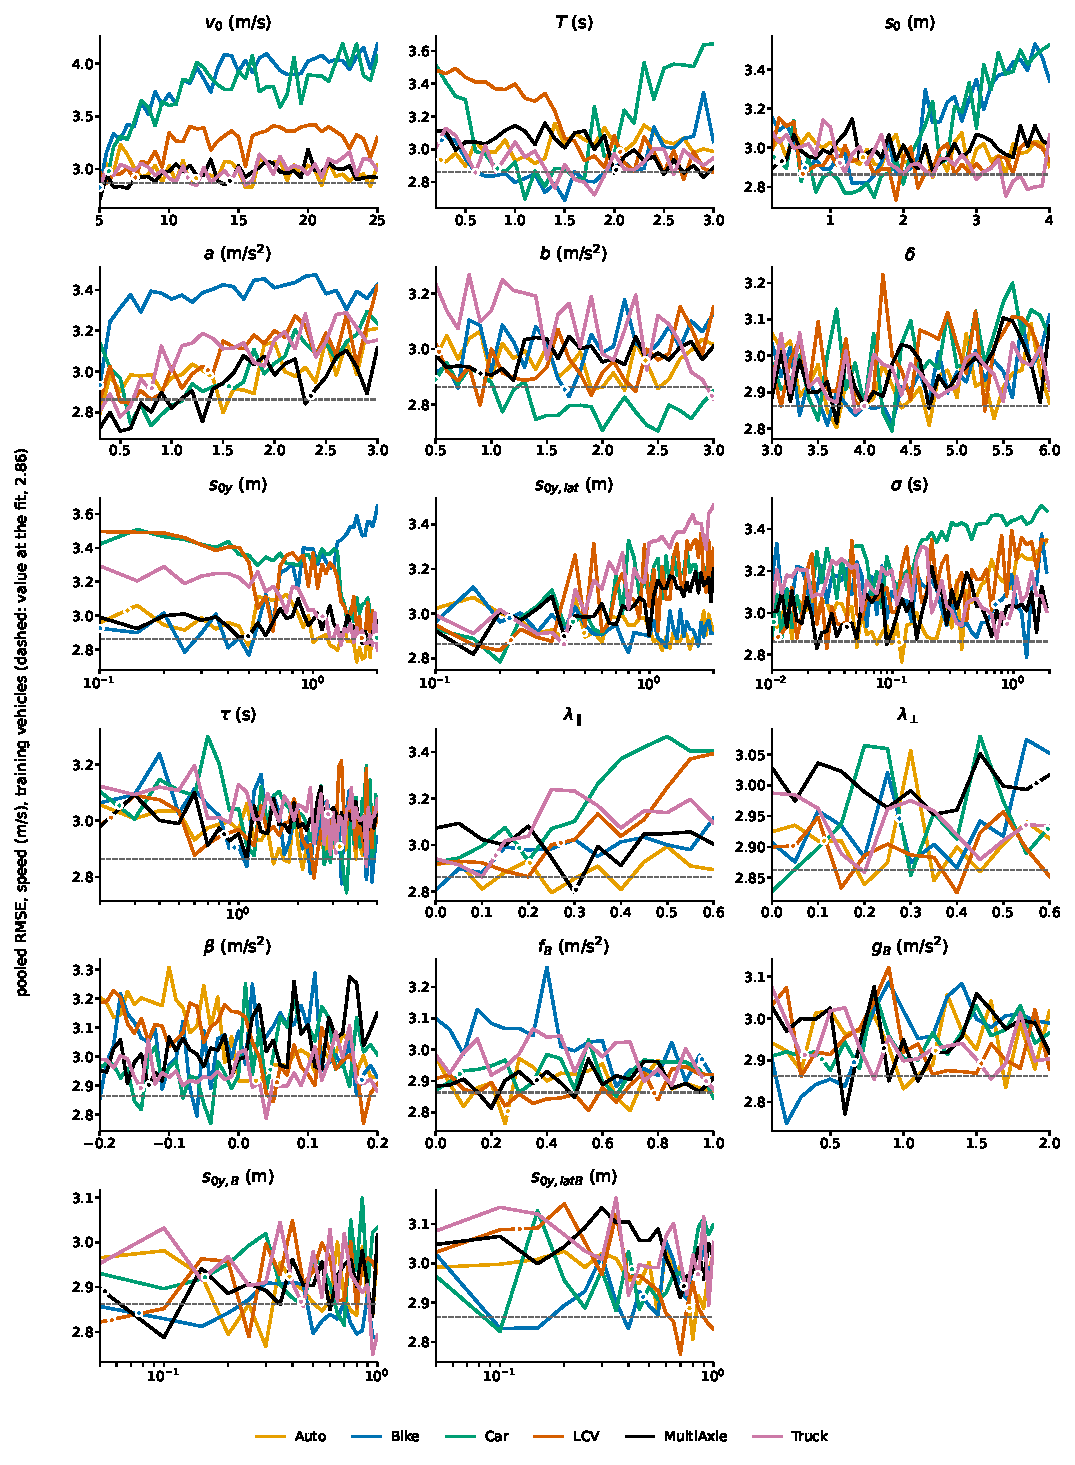
\includegraphics[width=\textwidth,height=0.85\textheight,keepaspectratio]{fig_oat_prof_speed.pdf}
\caption{Profiles as in Figure~\ref{fig:profF}, for the pooled RMSE of speed of
the training vehicles.}
\label{fig:profspeed}
\end{figure}

\section{Evidence for a signal beyond the exit}
\label{app:signal}
In the measured data the vehicles in the last 20\,m of the section stand still
during six periods, a stop roughly every 147\,s (coefficient of variation
$4\,\%$). Each queue starts at the exit and grows backwards. During the stops,
1.7 non-Bike vehicles per minute leave the section against 27.2 otherwise,
while Bikes keep leaving. The autocorrelation of mean speed at the exit peaks
at a lag of about 145\,s ($r=0.61$), more weakly upstream, and after each stop
the restart travels back up the queue at about 4--5\,m/s. This is the
behaviour of a signal, or an equivalent on/off restriction, at or beyond the
end of the recorded section (Figure~\ref{fig:signal}). An open-exit simulation
cannot form these queues, which is why the stop line is part of the set-up.

\begin{figure}[H]\centering
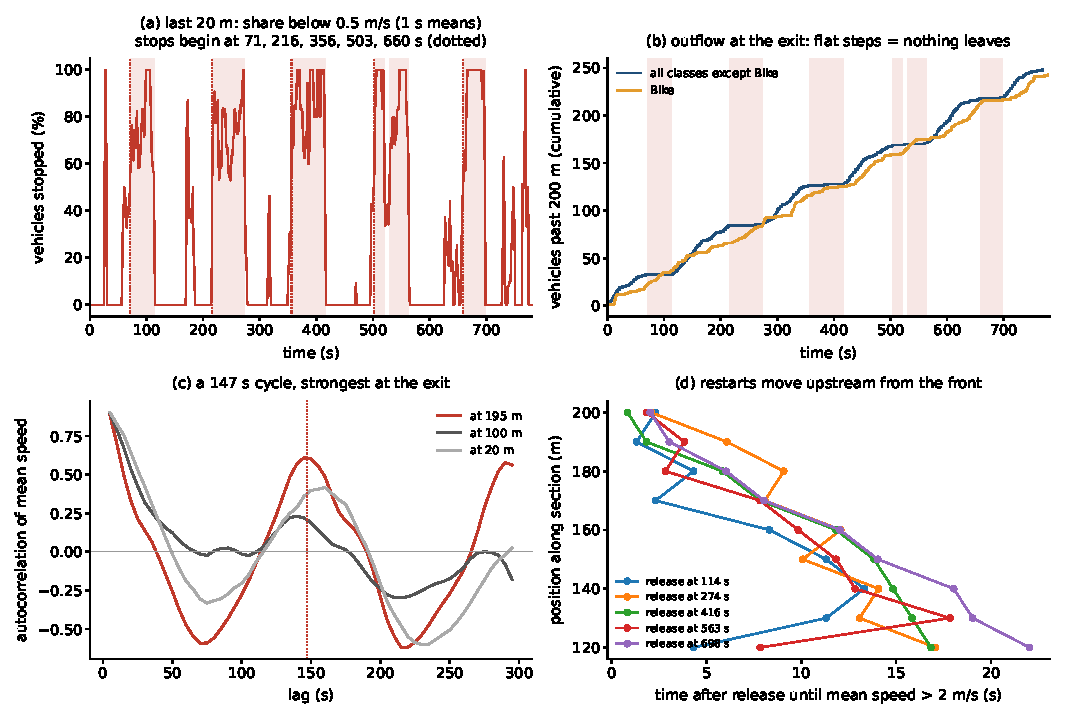
\includegraphics[width=0.68\textwidth]{fig_exit_signal.pdf}
\caption{Measured data only. Red bands: periods when the traffic at the exit is
stopped, also the periods when the stop line is on. (a) Share of vehicles in
the last 20\,m that are stopped. (b) Cumulative count of vehicles past 200\,m,
Bikes and all other classes. (c) Autocorrelation of mean speed against lag at
three positions. (d) Time after each stop ends until the traffic at each
position moves again.}
\label{fig:signal}
\end{figure}

\section{Simulation details}
\label{app:sim}
\paragraph{Neighbours.} Every vehicle within $\pm80$\,m longitudinally and
$\pm8$\,m laterally of the ego is a candidate neighbour, held in a list of 96
slots filled nearest first; in the measured traffic at most 64 vehicles are ever
inside one window, so no neighbour is missed. A neighbour acts only if its force
exceeds $b_{\mathrm{crit}}=0.1$\,m/s$^2$, a follower only within 0.5\,m.

\paragraph{Time step.} Each step of 0.04\,s computes all accelerations from the
same snapshot, updates speeds by explicit Euler, applies the heading
limit~\eqref{eq:clamp}, and updates positions by the trapezoid rule. A vehicle
whose speed would become negative stops instead and never reverses.

\paragraph{Leaving the section.} A simulated vehicle leaves when its centroid
crosses the end of the section, not when its measured twin leaves. If the twin
is still present it is held at the exit line and scored there.

\paragraph{Classes.} A class with fewer than ten vehicles shares the parameter
vector of the dimensionally nearest class with enough data; only Trailer does,
and it shares MultiAxle's.

\paragraph{Self-check.} Every fit ends by re-simulating the saved parameters and
recomputing the objective; a fit that does not reproduce the optimiser's best
value to six decimal places is rejected. All runs reported here pass.

\begin{longtable}{@{}lp{9.5cm}l@{}}
\caption{Fixed constants of the model and of the simulation.}\label{tab:const}\\
\toprule constant & meaning & value\\\midrule\endfirsthead
\toprule constant & meaning & value\\\midrule\endhead
$b_{\max}$ & maximum braking & 9 m/s$^2$\\
$b_{\mathrm{crit}}$ & force a neighbour must exceed to act & 0.1 m/s$^2$\\
$s_{\mathrm{follow}}$ & largest gap at which a follower pushes & 0.5 m\\
$0.2$ & reduction of the longitudinal force when side by side & --\\
$0.99$ & ACC weight of the IDM/CAH mix against plain IDM & --\\
$4b$ & limit on one neighbour's lateral acceleration & m/s$^2$\\
$\theta_{\max},\ \dot\theta_{\max}$ & heading cap and its rate limit & 0.3, 0.3 s$^{-1}$\\
$v_{\mathrm{ref}}$ & reference speed of the edge terms & 20 m/s\\
road edges & drivable span across the road & $y\in[0,8.9]$ m\\
stop line & position of the virtual stop line & 202.1 m\\
$\mathrm{d}t$ & time step, equal to the sampling interval & 0.04 s\\
$x_{\mathrm{sc}},\ y_{\mathrm{sc}}$ & error scales in $F$ & 2.0 m, 0.5 m\\
\bottomrule
\end{longtable}

\section{Vehicle dimensions and overlaps}
\label{app:dims}
Table~\ref{tab:dimcmp} compares the dimensions used here with those of the
earlier runs, and the overlaps of the measured vehicle rectangles that each
implies (every fifth frame). The reduction comes mainly from the smaller LCV:
LCV--LCV overlapping pair-frames fall from 530 to 17 and Car--LCV from 420 to
13. Pairs involving the wider Truck increase (Truck--Truck 233 to 391, Car--Truck
27 to 130).

\begin{table}[H]\centering\footnotesize
\caption{Earlier and current class dimensions, and overlaps of the measured
vehicle rectangles.}
\label{tab:dimcmp}
\begin{tabular}{@{}lcc@{}}
\toprule
& earlier & current\\
\midrule
Auto $L\times W$ (m) & $3.2\times1.4$ & $2.7\times1.4$\\
Bike & $1.8\times0.6$ & $1.8\times0.65$\\
Car & $4.0\times1.7$ & $4.0\times1.7$\\
LCV & $5.5\times2.0$ & $4.5\times1.75$\\
Truck & $8.2\times2.3$ & $8.5\times2.4$\\
MultiAxle & $12.5\times2.5$ & $12.0\times2.5$\\
Trailer & $16.3\times2.5$ & $15.5\times2.5$\\
\midrule
vehicle-frames in an overlap & $4.3\,\%$ & $3.0\,\%$\\
frames with any overlap & $57\,\%$ & $45\,\%$\\
vehicles that ever overlap & $42\,\%$ & $38\,\%$\\
overlapping pair-frames & 3\,844 & 2\,585\\
\bottomrule
\end{tabular}
\end{table}

\section{Errors by class}
\label{app:cls}
\begin{table}[H]\centering\footnotesize
\caption{Fixed IDM, single set \cite{chandra}: mean $F$ and pooled RMSE by class
(long.\ and lat.\ in m, speed in m/s).}
\begin{tabular}{@{}l rrrrr rrrrr@{}}\toprule
 & \multicolumn{5}{c}{training} & \multicolumn{5}{c}{held out}\\
\cmidrule(lr){2-6}\cmidrule(l){7-11}
class & $n$ & $F$ & long. & lat. & speed & $n$ & $F$ & long. & lat. & speed\\\midrule
Auto & 22 & 18.56 & 33.0 & 1.90 & 6.36 & 10 & 21.44 & 37.0 & 2.39 & 7.30\\
Bike & 178 & 21.64 & 37.4 & 2.41 & 6.03 & 76 & 21.68 & 37.8 & 2.24 & 5.65\\
Car & 87 & 16.75 & 29.7 & 1.76 & 7.14 & 37 & 17.82 & 31.1 & 1.44 & 6.47\\
LCV & 46 & 20.63 & 38.1 & 1.13 & 6.19 & 20 & 19.07 & 32.7 & 1.00 & 7.25\\
Truck & 36 & 19.36 & 37.7 & 1.51 & 9.14 & 15 & 19.71 & 39.1 & 1.03 & 6.76\\
MultiAxle & 13 & 23.67 & 37.1 & 1.04 & 8.51 & 5 & 16.94 & 35.7 & 0.85 & 4.97\\
Trailer & 4 & 18.30 & 41.9 & 0.66 & 10.72 & 2 & 24.97 & 46.1 & 0.65 & 3.56\\
\midrule all & 386 & 20.06 & 35.1 & 1.89 & 6.97 & 165 & 20.20 & 35.5 & 1.73 & 6.35\\
\bottomrule\end{tabular}

\end{table}
\begin{table}[H]\centering\footnotesize
\caption{Fixed IDM, per class \cite{duggal}: mean $F$ and pooled RMSE by class.}
\begin{tabular}{@{}l rrrrr rrrrr@{}}\toprule
 & \multicolumn{5}{c}{training} & \multicolumn{5}{c}{held out}\\
\cmidrule(lr){2-6}\cmidrule(l){7-11}
class & $n$ & $F$ & long. & lat. & speed & $n$ & $F$ & long. & lat. & speed\\\midrule
Auto & 22 & 26.51 & 47.2 & 1.82 & 13.02 & 10 & 32.47 & 53.2 & 2.29 & 13.42\\
Bike & 178 & 25.92 & 45.8 & 2.35 & 9.76 & 76 & 28.46 & 51.6 & 2.15 & 8.95\\
Car & 87 & 24.43 & 44.5 & 1.28 & 12.63 & 37 & 23.34 & 42.3 & 1.19 & 11.71\\
LCV & 46 & 28.60 & 53.9 & 1.13 & 11.18 & 20 & 26.35 & 46.2 & 0.89 & 12.32\\
Truck & 36 & 26.96 & 51.8 & 1.30 & 11.96 & 15 & 28.64 & 53.6 & 1.43 & 11.00\\
MultiAxle & 13 & 28.32 & 46.2 & 2.05 & 9.30 & 5 & 26.77 & 55.9 & 1.23 & 9.38\\
Trailer & 4 & 17.84 & 40.9 & 0.83 & 9.55 & 2 & 35.48 & 71.7 & 0.95 & 4.26\\
\midrule all & 386 & 26.03 & 47.5 & 1.76 & 11.35 & 165 & 27.35 & 49.3 & 1.65 & 10.87\\
\bottomrule\end{tabular}

\end{table}
\begin{table}[H]\centering\footnotesize
\caption{All parameters free: mean $F$ and pooled RMSE by class.}
\begin{tabular}{@{}l rrrrr rrrrr@{}}\toprule
 & \multicolumn{5}{c}{training} & \multicolumn{5}{c}{held out}\\
\cmidrule(lr){2-6}\cmidrule(l){7-11}
class & $n$ & $F$ & long. & lat. & speed & $n$ & $F$ & long. & lat. & speed\\\midrule
Auto & 22 & 14.49 & 24.5 & 1.80 & 2.83 & 10 & 15.30 & 23.8 & 2.74 & 2.19\\
Bike & 178 & 13.76 & 23.8 & 1.81 & 2.83 & 76 & 13.43 & 27.0 & 1.69 & 2.69\\
Car & 87 & 10.61 & 20.1 & 1.11 & 2.73 & 37 & 10.60 & 18.1 & 1.21 & 2.62\\
LCV & 46 & 10.98 & 21.0 & 1.14 & 2.11 & 20 & 10.52 & 20.2 & 0.97 & 2.78\\
Truck & 36 & 12.17 & 24.3 & 1.59 & 2.85 & 15 & 10.88 & 21.2 & 1.25 & 2.51\\
MultiAxle & 13 & 11.52 & 19.5 & 0.72 & 4.76 & 5 & 9.20 & 15.1 & 0.87 & 2.29\\
Trailer & 4 & 12.22 & 28.3 & 0.73 & 5.88 & 2 & 12.45 & 20.0 & 0.97 & 1.74\\
\midrule all & 386 & 12.52 & 22.3 & 1.47 & 2.86 & 165 & 12.19 & 22.4 & 1.51 & 2.60\\
\bottomrule\end{tabular}

\end{table}

\section{Convergence}
\label{app:conv}
Each panel shows the training objective against the number of objective
evaluations (one evaluation is one simulation of the whole record) and the
CMA-ES step size $\sigma_{\mathrm{c}}$ below.

A \emph{generation} is one iteration of CMA-ES: it draws $\lambda$ candidate
parameter sets around the current mean (17 for the free fit, 16 for the
fixed-IDM fits), simulates the record once for each, ranks them by $F$ and
updates the mean, step size and covariance. One generation therefore costs
$\lambda$ evaluations; the free fit ran about 1\,240 generations. The curves are:
\begin{itemize}\setlength{\itemsep}{1pt}
\item \emph{best of each generation}: the lowest $F$ among that generation's
$\lambda$ candidates. It fluctuates, since every generation is a new random
draw;
\item \emph{median of each generation}: the middle $F$ of the $\lambda$
candidates, a measure of where the search distribution as a whole stands;
\item \emph{best so far}: the lowest $F$ found up to that point, which can only
fall and is the value the fit returns.
\end{itemize}
Early in a run the median lies far above the best, because the distribution is
wide and many candidates are poor; as the search narrows, the median closes in
on the best. A run has settled when the best so far no longer falls, the median
has come down to it and the step size keeps shrinking.

\begin{figure}[H]\centering
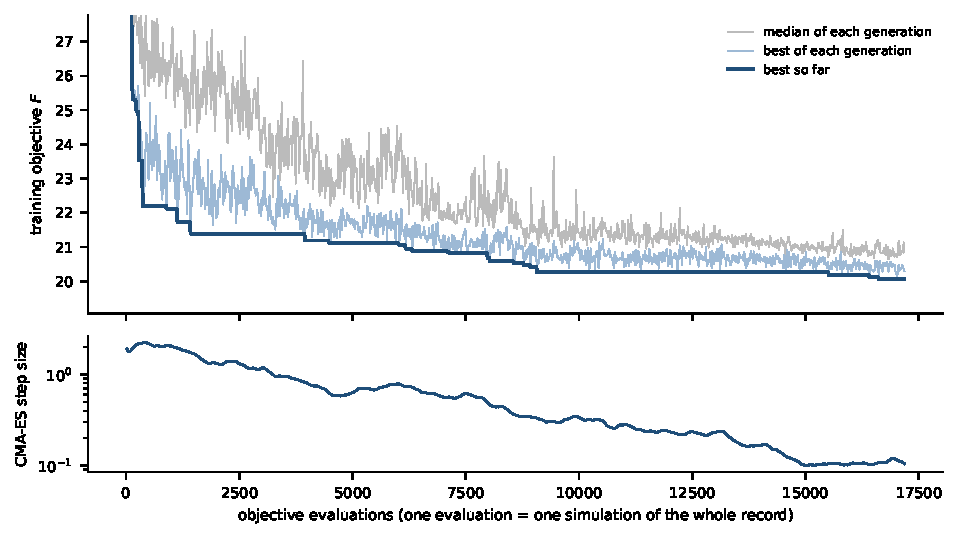
\includegraphics[width=0.8\textwidth]{fig_conv_chandra.pdf}
\caption{Convergence, fixed IDM, single set \cite{chandra}.}
\end{figure}
\begin{figure}[H]\centering
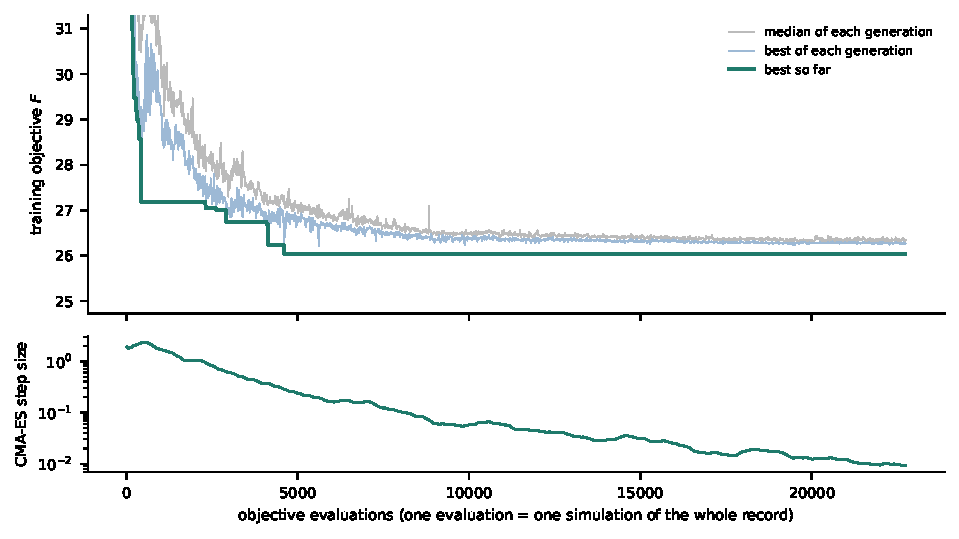
\includegraphics[width=0.8\textwidth]{fig_conv_duggal.pdf}
\caption{Convergence, fixed IDM, per class \cite{duggal}.}
\end{figure}
\begin{figure}[H]\centering
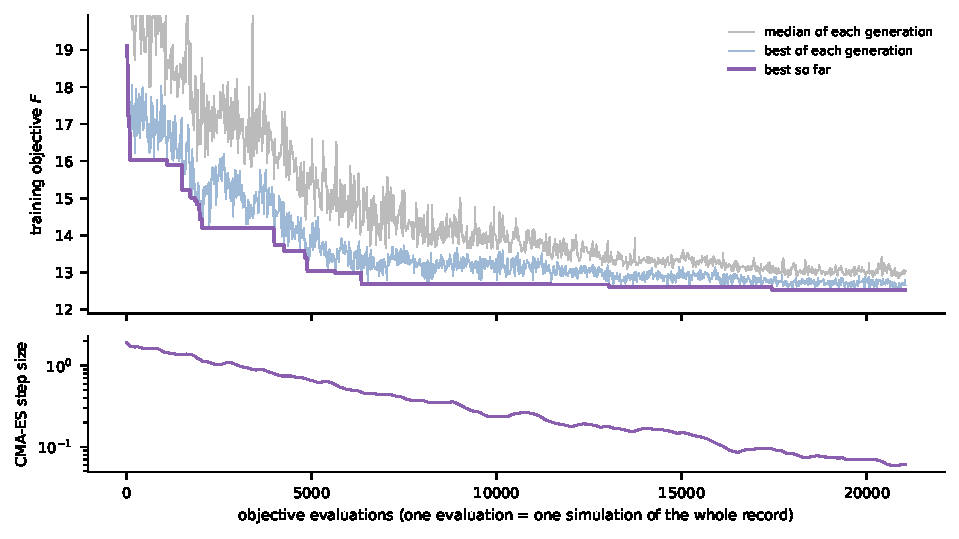
\includegraphics[width=0.8\textwidth]{fig_conv_free.pdf}
\caption{Convergence, all parameters free.}
\end{figure}

\end{document}
